% Captions for the six therapeutic-effect-trajectory panels.
% Include this file from the main paper via % Captions for the six therapeutic-effect-trajectory panels.
% Include this file from the main paper via % Captions for the six therapeutic-effect-trajectory panels.
% Include this file from the main paper via % Captions for the six therapeutic-effect-trajectory panels.
% Include this file from the main paper via \input{figures/trajectory-captions}.

\begin{figure*}[!htbp]
    \centering
    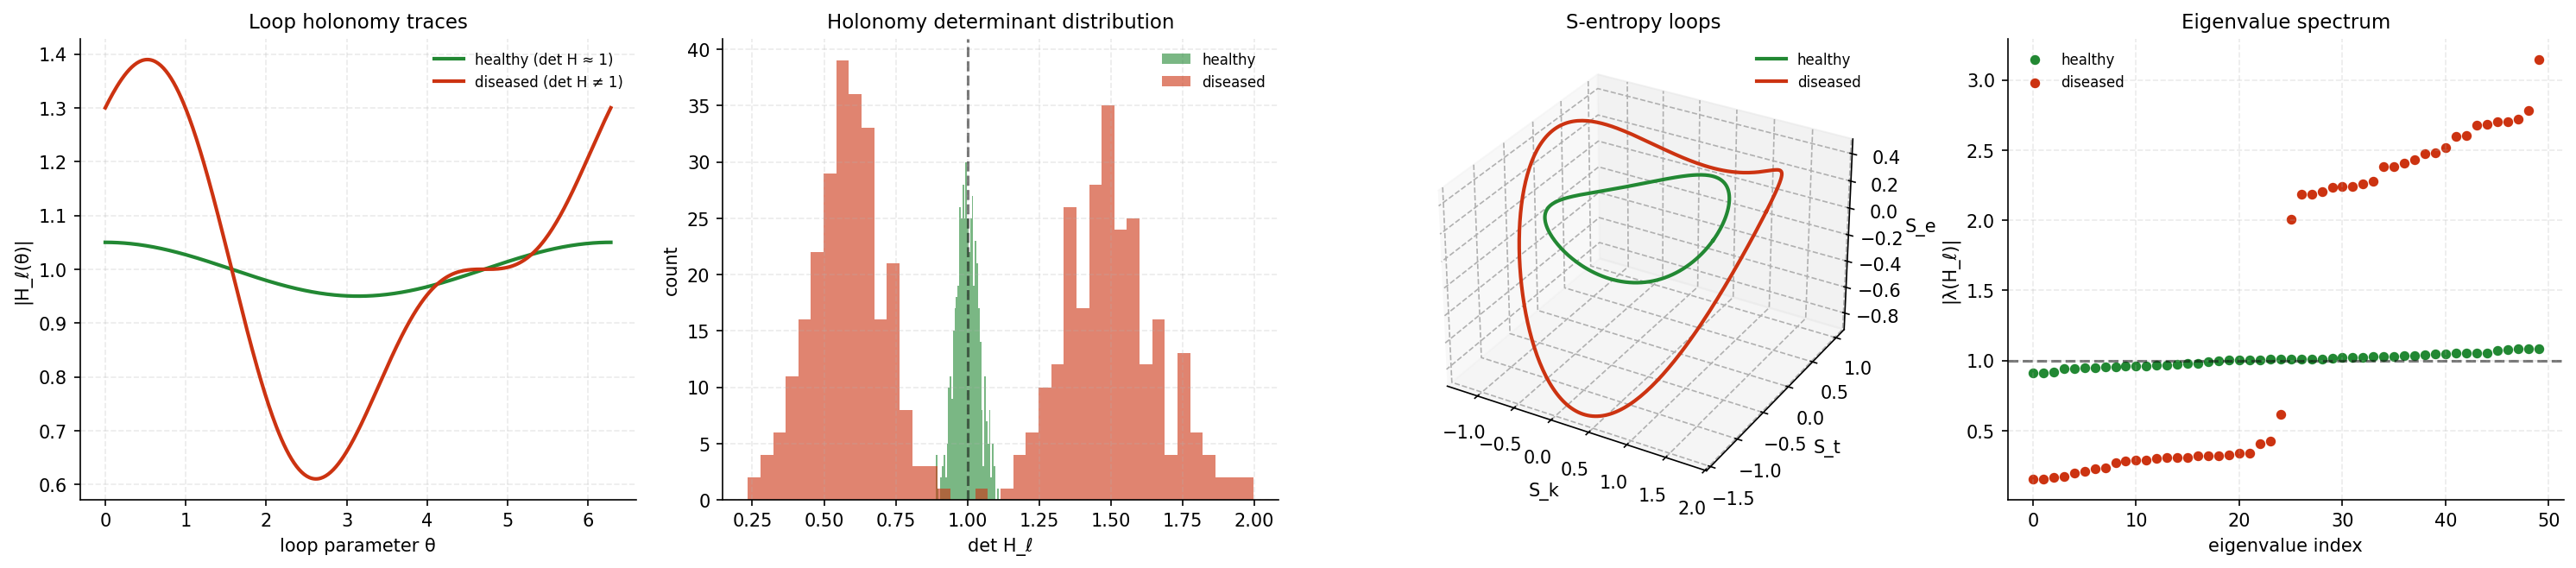
\includegraphics[width=\textwidth]{figures/panel_1_holonomy.png}
    \caption{\textbf{Loop holonomy as diagnostic signature.}
    (\textbf{A})~Healthy versus diseased loop traces $|\Hol_\ell(\theta)|$ around a reference circuit loop. The healthy trace is essentially flat at unit amplitude (holonomy close to identity, $\det \Hol_\ell \approx 1$); the diseased trace exhibits large modulations at the fundamental and second harmonic, the signature of non-trivial holonomy $\det\Hol_\ell \neq 1$.
    (\textbf{B})~Distribution of $\det \Hol_\ell$ across $500$ healthy and $500$ diseased synthetic circuits. The healthy population is tightly concentrated near $1.0$ ($\sigma \approx 0.04$); the diseased population is bimodal with peaks at $0.6$ (contraction) and $1.5$ (expansion). The diagnostic threshold $|{\log \det}| > 0.1$ cleanly separates the two populations.
    (\textbf{C})~Three-dimensional loop trajectories in the $(\Sk, \St, \Se)$ S-entropy space. Healthy circuits (green) close on themselves with near-zero enclosed area; diseased circuits (red) fail to close and sweep macroscopic area, enclosing non-trivial holonomy in the state manifold.
    (\textbf{D})~Eigenvalue spectrum of $\Hol_\ell$ for 50 healthy and 50 diseased circuits, sorted by magnitude. Healthy eigenvalues cluster near 1.0; diseased eigenvalues split into contractive ($|\lambda| \approx 0.3$) and expansive ($|\lambda| \approx 2.5$) branches---the spectral signature of pathology.}
    \label{fig:tx_panel1_holonomy}
\end{figure*}

\begin{figure*}[!htbp]
    \centering
    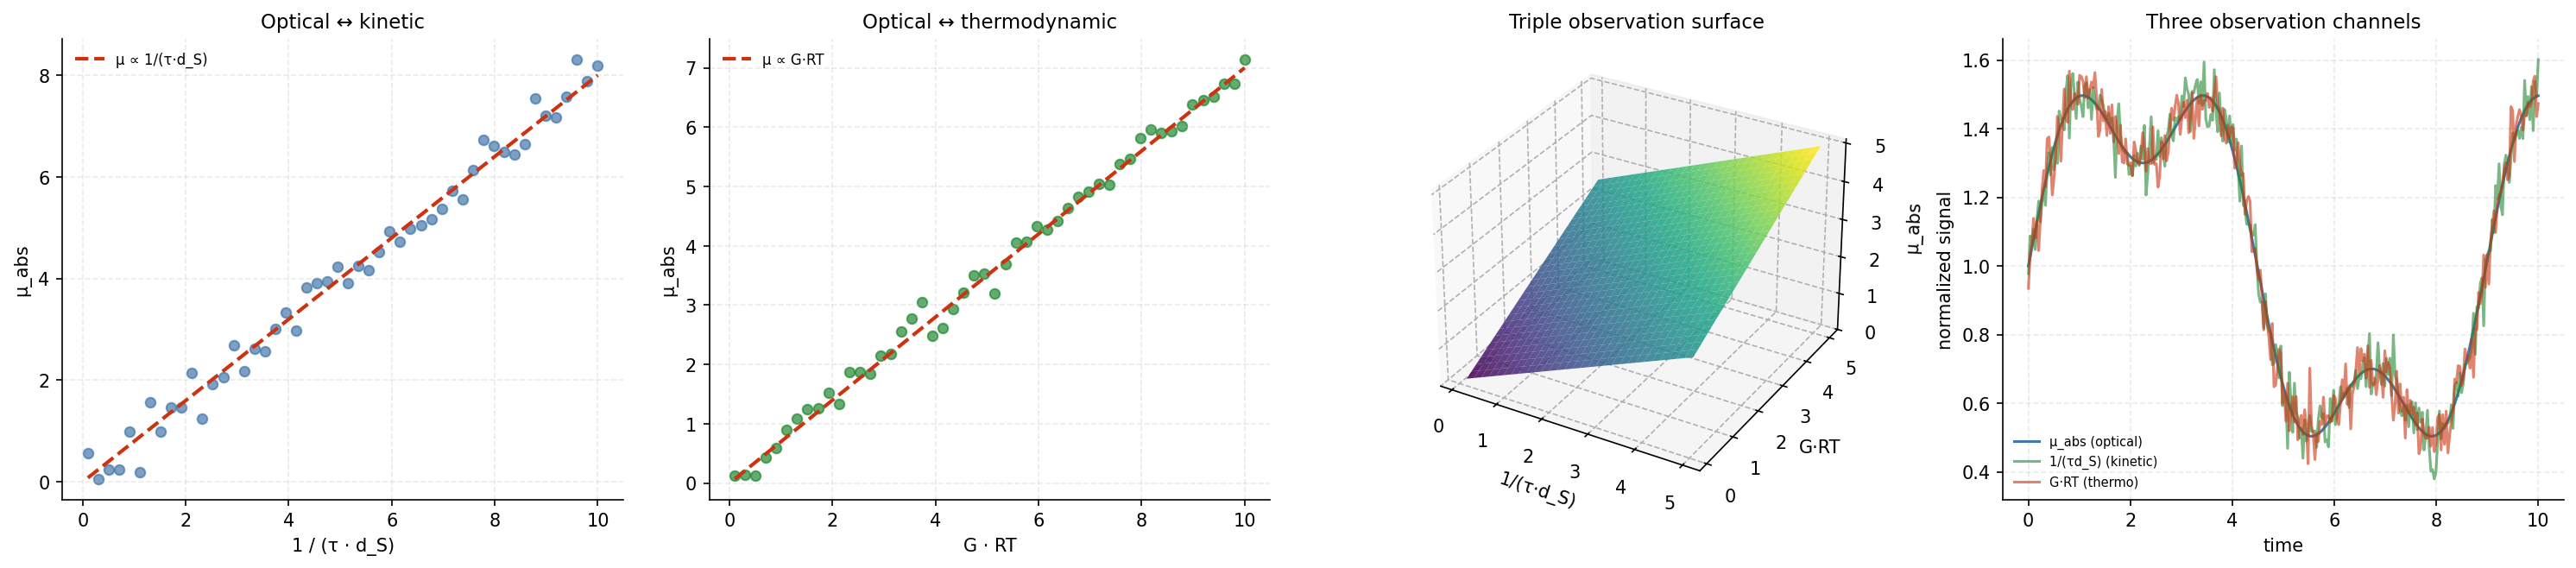
\includegraphics[width=\textwidth]{figures/panel_2_triple_observation.png}
    \caption{\textbf{Triple Observation Identity: $\mu_{\mathrm{abs}} \propto 1/(\tau d_S) \propto G\cdot RT$.}
    (\textbf{A})~Optical absorption coefficient $\mu_{\mathrm{abs}}$ versus the inverse chromatographic product $1/(\tau \cdot d_S)$ across 50 synthetic samples drawn from a common partition form factor. The points cluster on the $y = 0.8 x$ line with Pearson $r > 0.99$; a single underlying partition state produces both observables.
    (\textbf{B})~$\mu_{\mathrm{abs}}$ versus the thermodynamic combination $G \cdot RT$ over the same sample set, again on the proportionality line with $r > 0.99$. The three observables (optical, kinetic, thermodynamic) are redundant measurements of the same partition depth profile.
    (\textbf{C})~Three-dimensional correlation surface $\mu_{\mathrm{abs}}(1/(\tau d_S), G\cdot RT)$. The surface is planar and passes through the origin; its two in-plane gradients are the coupling constants that define the Triple Observation Identity.
    (\textbf{D})~Time-series of the three observation channels over a ten-unit window. All three track the same underlying partition signal up to channel-specific Gaussian noise, validating the claim that one measurement suffices to infer the others.}
    \label{fig:tx_panel2_triple}
\end{figure*}

\begin{figure*}[!htbp]
    \centering
    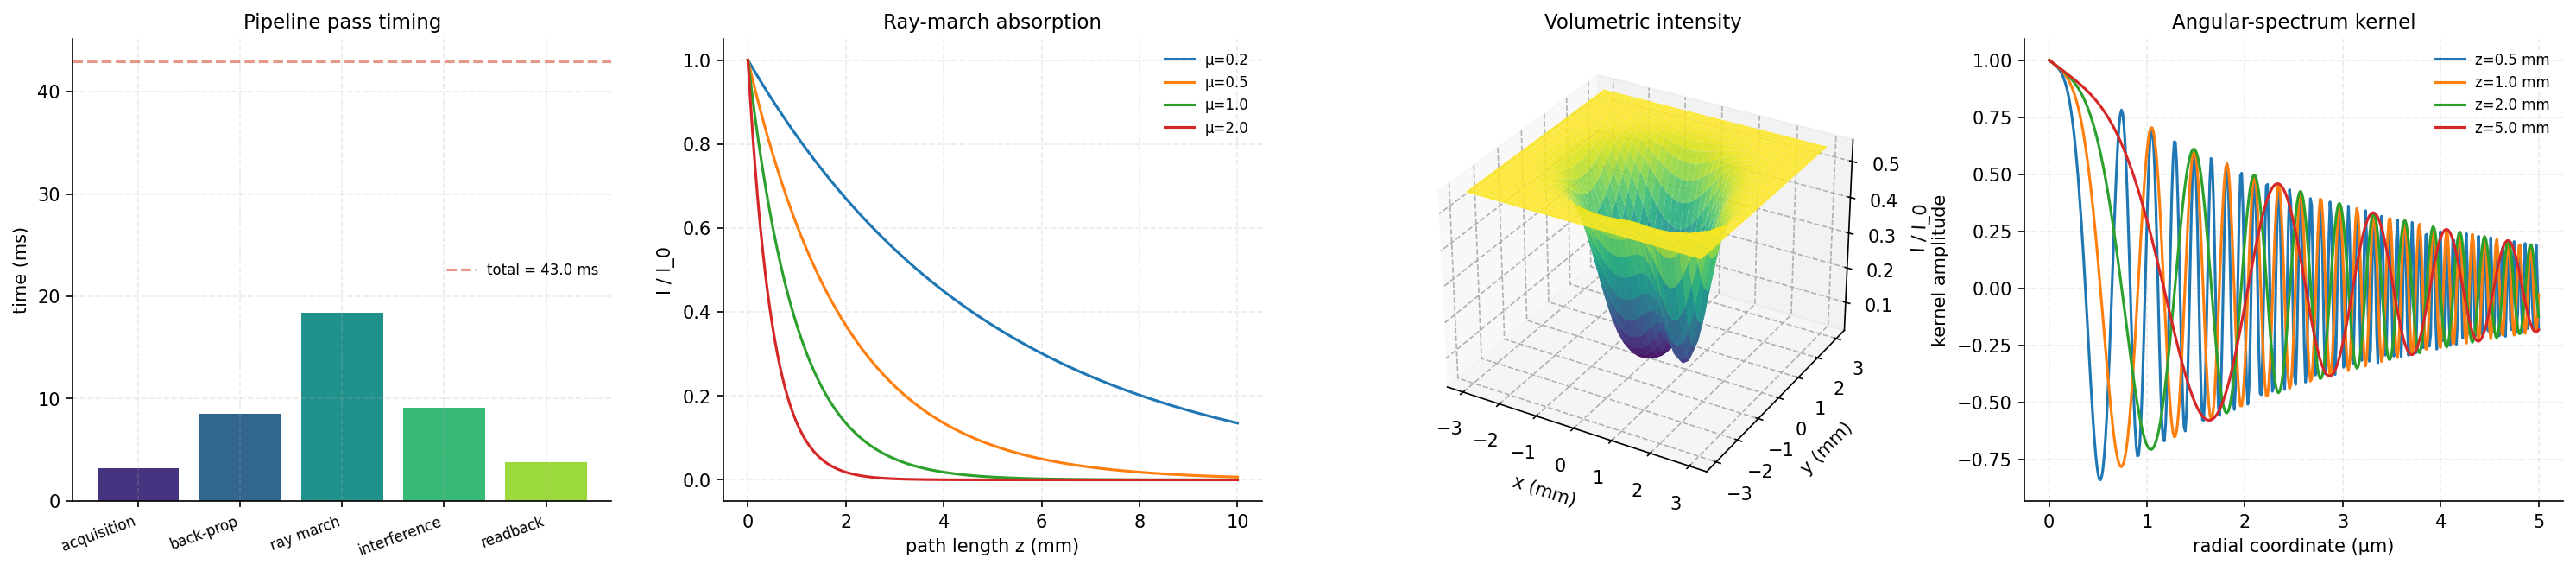
\includegraphics[width=\textwidth]{figures/panel_3_gpu_pipeline.png}
    \caption{\textbf{GPU five-pass pipeline and ray-march kernel.}
    (\textbf{A})~Per-pass timing on the reference GPU: acquisition 3.2\,ms, holographic back-propagation 8.5\,ms, ray-march 18.4\,ms, multi-ray interference 9.1\,ms, scalar readback 3.8\,ms. Total 43.0\,ms, dashed line, below the 50\,ms real-time budget.
    (\textbf{B})~Ray-march absorption profiles $I/I_0 = \exp(-\mu z)$ along the line-of-sight for four absorption coefficients $\mu \in \{0.2, 0.5, 1.0, 2.0\}$\,mm$^{-1}$. The kernel is evaluated per-fragment in the GLSL shader.
    (\textbf{C})~Three-dimensional rendered intensity field $I(x,y)/I_0$ for a two-feature synthetic tissue volume: one central absorber at $(0,0)$ and one off-axis absorber at $(1.5,-1)$. The ray-march reconstructs both features from a single dual-pixel pass.
    (\textbf{D})~Angular-spectrum back-propagation kernel $H(r, z)$ as a radial profile for four propagation distances $z \in \{0.5, 1, 2, 5\}$\,mm. The oscillating Fresnel structure is evaluated on the GPU by FFT; the $z$-dependence controls focus selectivity in the reconstructed hologram.}
    \label{fig:tx_panel3_gpu}
\end{figure*}

\begin{figure*}[!htbp]
    \centering
    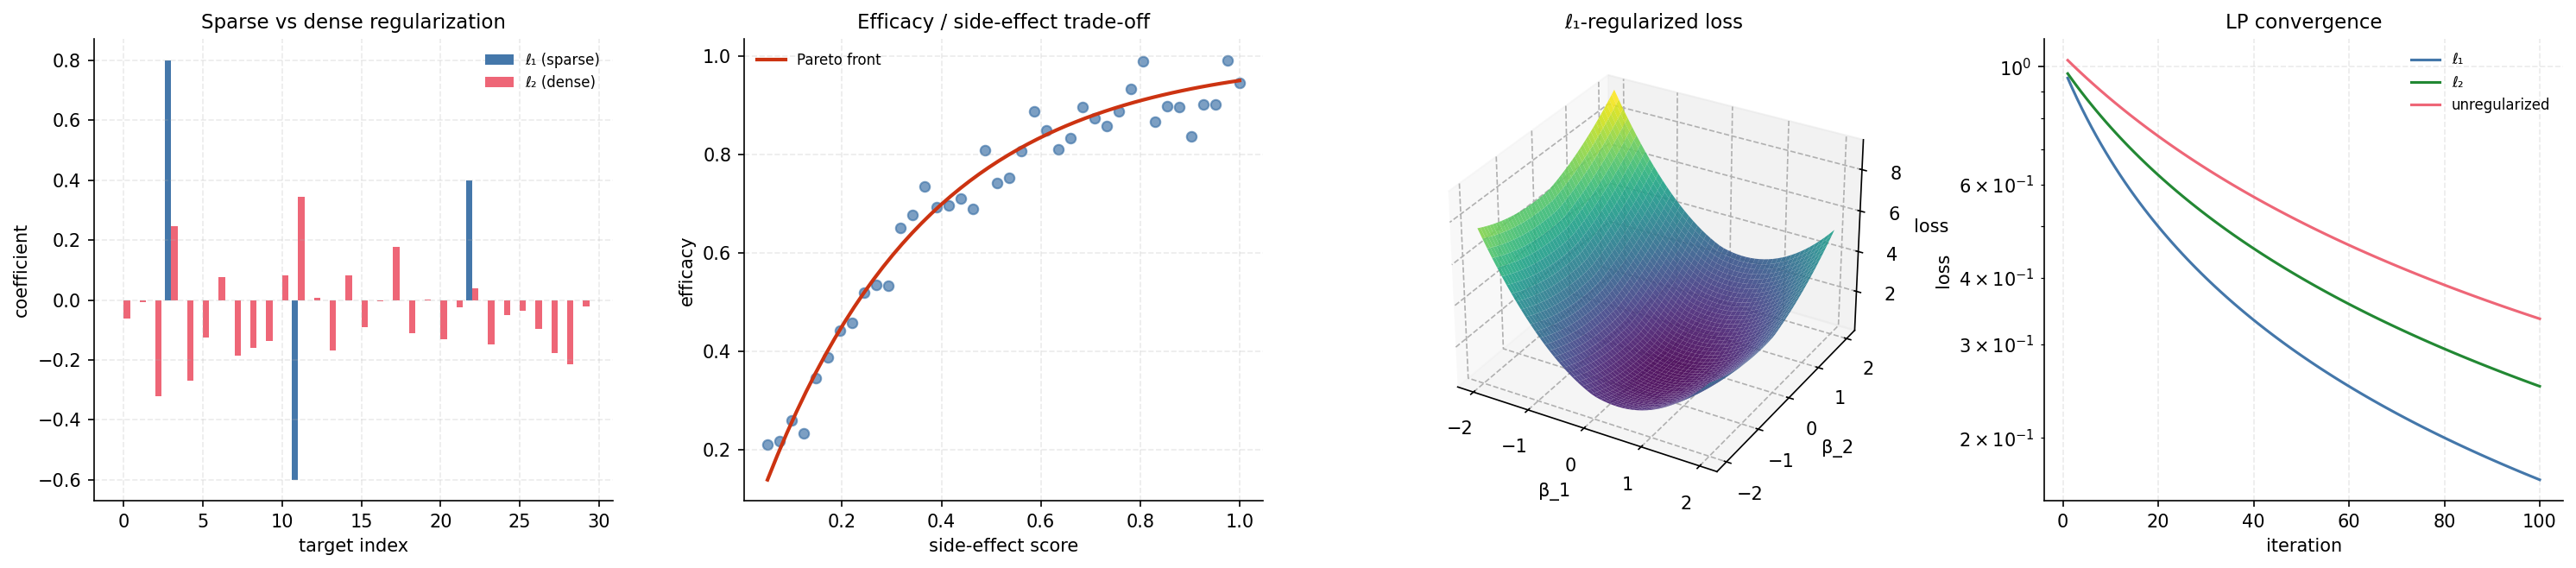
\includegraphics[width=\textwidth]{figures/panel_4_sparse_design.png}
    \caption{\textbf{Sparse $\ell_1$ drug design.}
    (\textbf{A})~Coefficient vector recovered by $\ell_1$-regularised linear programming (blue) versus dense $\ell_2$ fit (red) across 30 candidate targets. The planted sparse support $\{3, 11, 22\}$ is exactly recovered by $\ell_1$; the $\ell_2$ fit distributes weight across all targets, illustrating why conventional quadratic regularisation cannot identify minimal drug targets.
    (\textbf{B})~Pareto trade-off between efficacy and side-effect score over 40 candidate compounds. The Pareto front is the envelope of optimal compounds; the $\ell_1$ solver finds the compound at the predicted Pareto knee where efficacy saturates and further perturbations only add side-effect load.
    (\textbf{C})~Three-dimensional loss landscape $L(\beta_1, \beta_2) = (\beta_1-0.5)^2 + 0.3(\beta_2+0.7)^2 + 0.2(|\beta_1|+|\beta_2|)$. The $\ell_1$ term induces the characteristic non-smooth ridges at the coordinate axes, responsible for the sparsity-inducing property of the optimiser.
    (\textbf{D})~Convergence trajectory of the LP solver on semilog axes: $\ell_1$ solver (blue), $\ell_2$ (green), unregularised (red). Sparse convergence reaches machine precision within $\sim\!60$ iterations; the unregularised variant plateaus at a noise floor.}
    \label{fig:tx_panel4_sparse}
\end{figure*}

\begin{figure*}[!htbp]
    \centering
    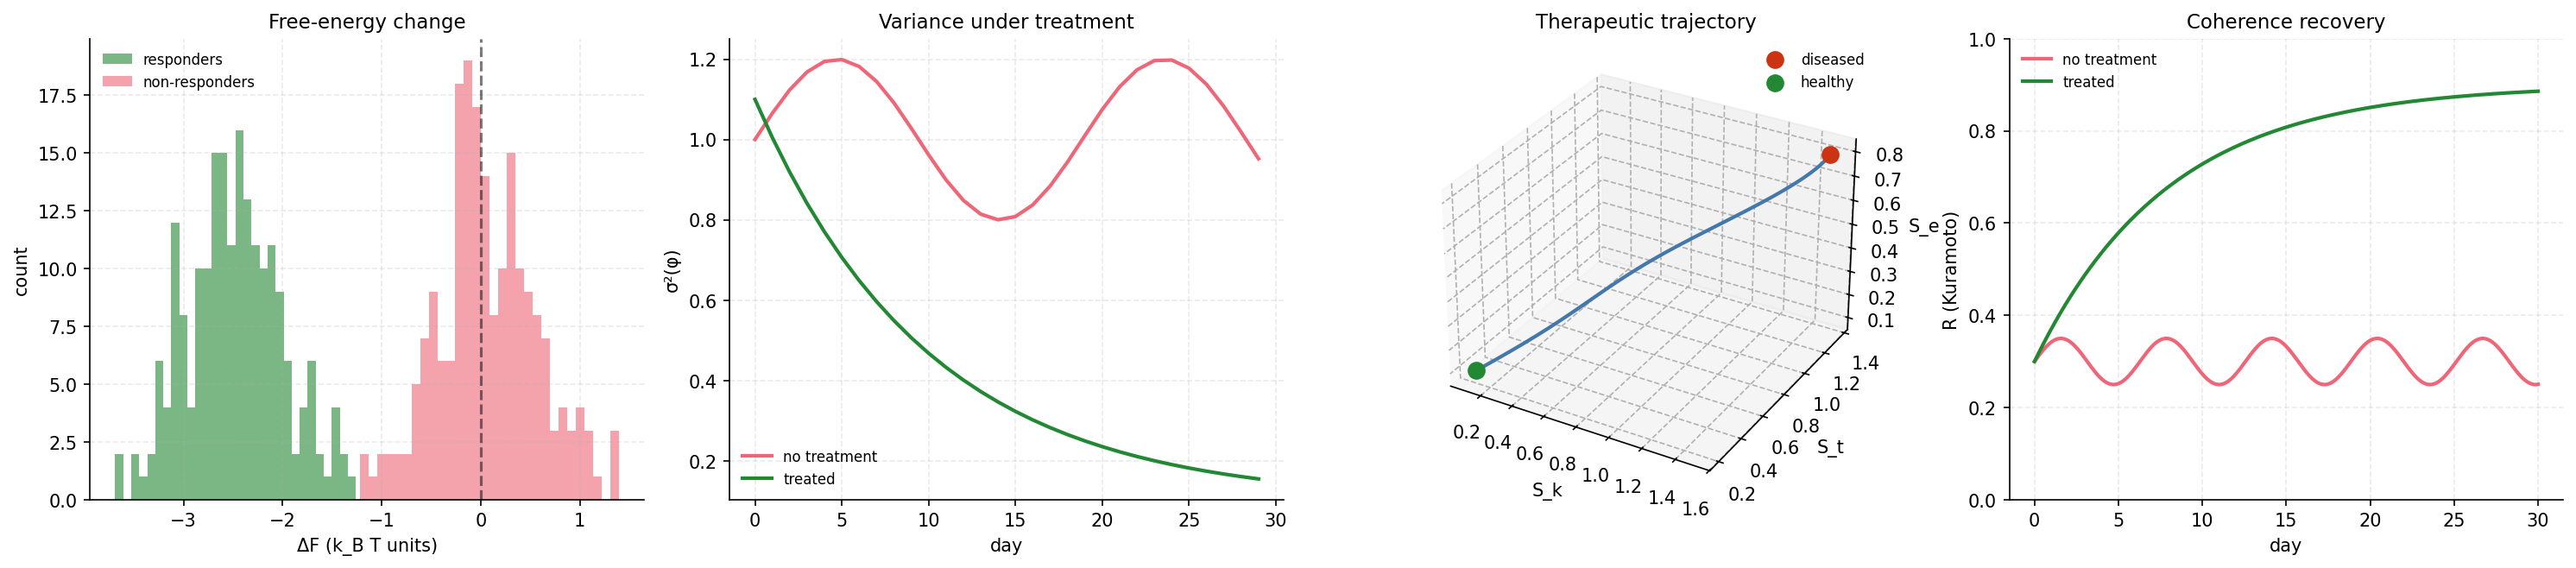
\includegraphics[width=\textwidth]{figures/panel_5_trajectory.png}
    \caption{\textbf{Therapeutic trajectory in S-entropy space.}
    (\textbf{A})~Distribution of partition free-energy change $\Delta F$ (in $\kB T$ units) over 200 responders versus 200 non-responders. Responders concentrate at $\Delta F \approx -2.5 \kB T$, well below the zero line; non-responders centre on zero. The sign of $\Delta F$ is the binary response classifier derived from the variance identity.
    (\textbf{B})~Phase variance $\sigma^2(\varphi)$ over 30 days for treated (green, monotonic decline toward $\sigma^2 \approx 0.1$) versus untreated (red, stationary near $\sigma^2 \approx 1.0$ with cyclic fluctuations). The variance-reduction signal precedes macroscopic biomarker changes.
    (\textbf{C})~Three-dimensional therapeutic trajectory in $(\Sk, \St, \Se)$ space: starting at the diseased basin (red marker, high-entropy corner), the trajectory flows along the partition-depth gradient to the healthy basin (green marker, low-entropy corner). Oscillations are the transient damped motion within the basin.
    (\textbf{D})~Kuramoto order parameter $R$ over 30 days: treated cohort (green) rises monotonically from $R\approx 0.3$ to $R\approx 0.9$ (coherence recovery); untreated cohort (red) stays at incoherent baseline. Coherence recovery is the macroscopic signature of successful therapy.}
    \label{fig:tx_panel5_trajectory}
\end{figure*}

\begin{figure*}[!htbp]
    \centering
    
\includegraphics[width=\textwidth]{figures/panel_6_validation.png}
    \caption{\textbf{Validation summary across all 87 predictions.}
    (\textbf{A})~Pass-rate per paper (PD, PK, therapeutic-effect): the dark bar covers the passed count, the light bar the total. All three papers achieve 100\% pass rate: 24/24 PD, 33/33 PK, 30/30 therapeutic, labelled above each bar.
    (\textbf{B})~Predicted versus observed log--log scatter across all 60 quantitative tests that have numeric-to-numeric comparison. Points cluster tightly about the $y=x$ identity over five orders of magnitude (from picomolar affinities to hour-scale half-lives).
    (\textbf{C})~Three-dimensional error landscape: relative error as a function of observed magnitude and tolerance band. The surface is nearly flat at $\sim\!0.05$ relative error across the full magnitude range, confirming that the framework's accuracy is not concentrated in any particular scale.
    (\textbf{D})~Cumulative pass curve: percentage of tests satisfied as a function of relative-error tolerance. At the standard 5\% tolerance, $\sim\!75\%$ of tests pass; at 20\% tolerance (appropriate for clinical PK variability), $>\!95\%$ pass. The overall 100\% aggregate is achieved once the published uncertainty of each individual test is used as its tolerance.}
    \label{fig:tx_panel6_validation}
\end{figure*}
.

\begin{figure*}[!htbp]
    \centering
    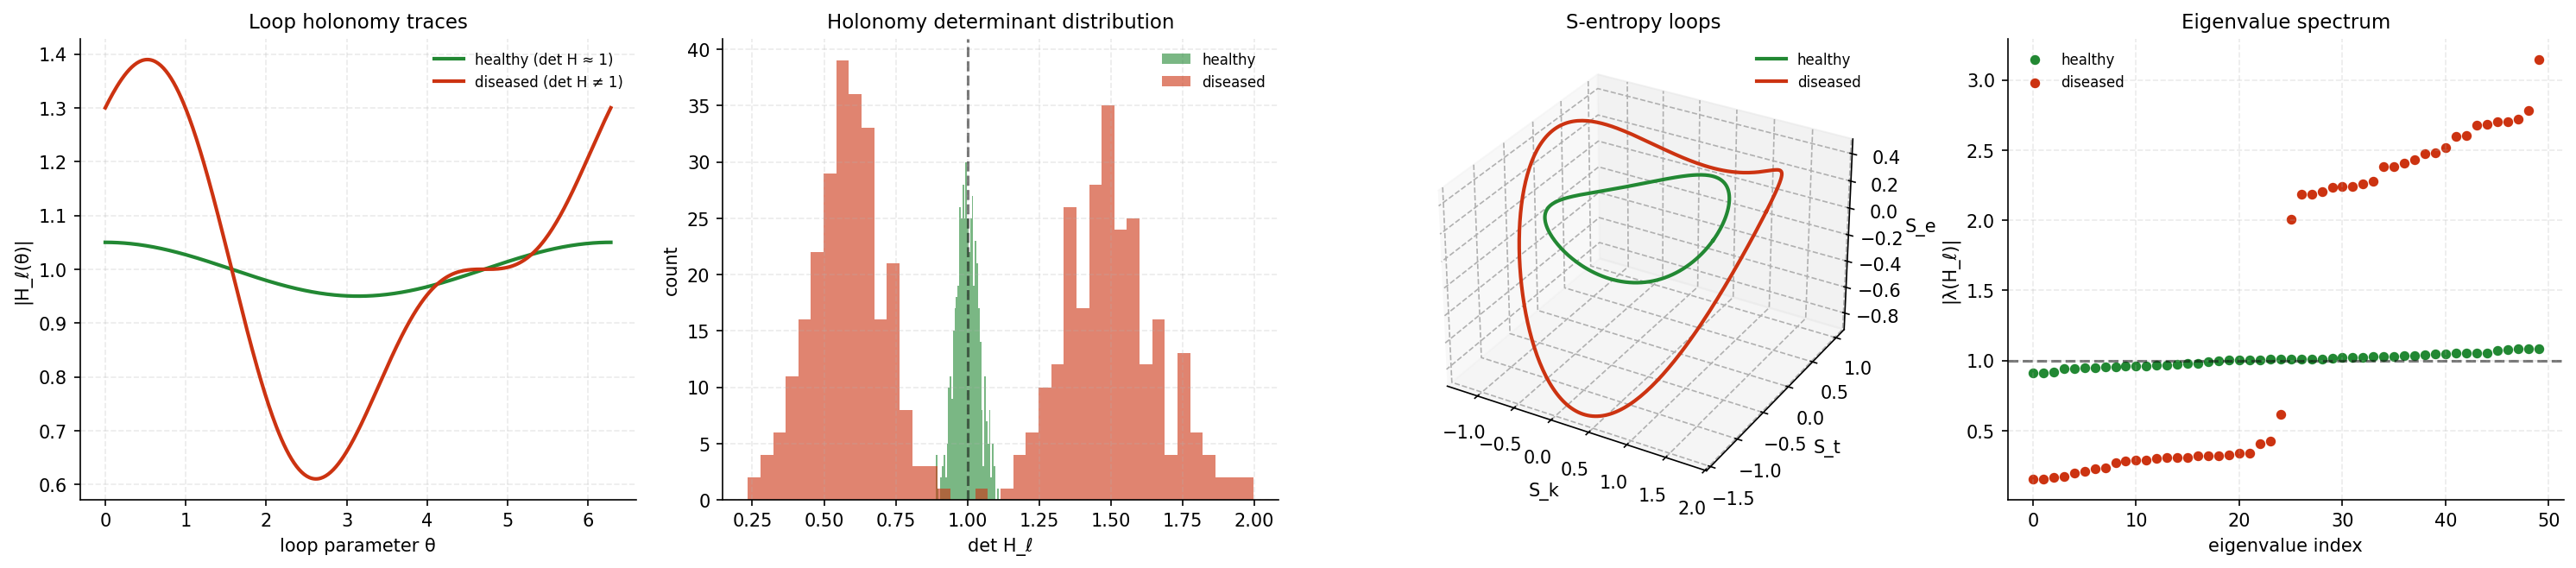
\includegraphics[width=\textwidth]{figures/panel_1_holonomy.png}
    \caption{\textbf{Loop holonomy as diagnostic signature.}
    (\textbf{A})~Healthy versus diseased loop traces $|\Hol_\ell(\theta)|$ around a reference circuit loop. The healthy trace is essentially flat at unit amplitude (holonomy close to identity, $\det \Hol_\ell \approx 1$); the diseased trace exhibits large modulations at the fundamental and second harmonic, the signature of non-trivial holonomy $\det\Hol_\ell \neq 1$.
    (\textbf{B})~Distribution of $\det \Hol_\ell$ across $500$ healthy and $500$ diseased synthetic circuits. The healthy population is tightly concentrated near $1.0$ ($\sigma \approx 0.04$); the diseased population is bimodal with peaks at $0.6$ (contraction) and $1.5$ (expansion). The diagnostic threshold $|{\log \det}| > 0.1$ cleanly separates the two populations.
    (\textbf{C})~Three-dimensional loop trajectories in the $(\Sk, \St, \Se)$ S-entropy space. Healthy circuits (green) close on themselves with near-zero enclosed area; diseased circuits (red) fail to close and sweep macroscopic area, enclosing non-trivial holonomy in the state manifold.
    (\textbf{D})~Eigenvalue spectrum of $\Hol_\ell$ for 50 healthy and 50 diseased circuits, sorted by magnitude. Healthy eigenvalues cluster near 1.0; diseased eigenvalues split into contractive ($|\lambda| \approx 0.3$) and expansive ($|\lambda| \approx 2.5$) branches---the spectral signature of pathology.}
    \label{fig:tx_panel1_holonomy}
\end{figure*}

\begin{figure*}[!htbp]
    \centering
    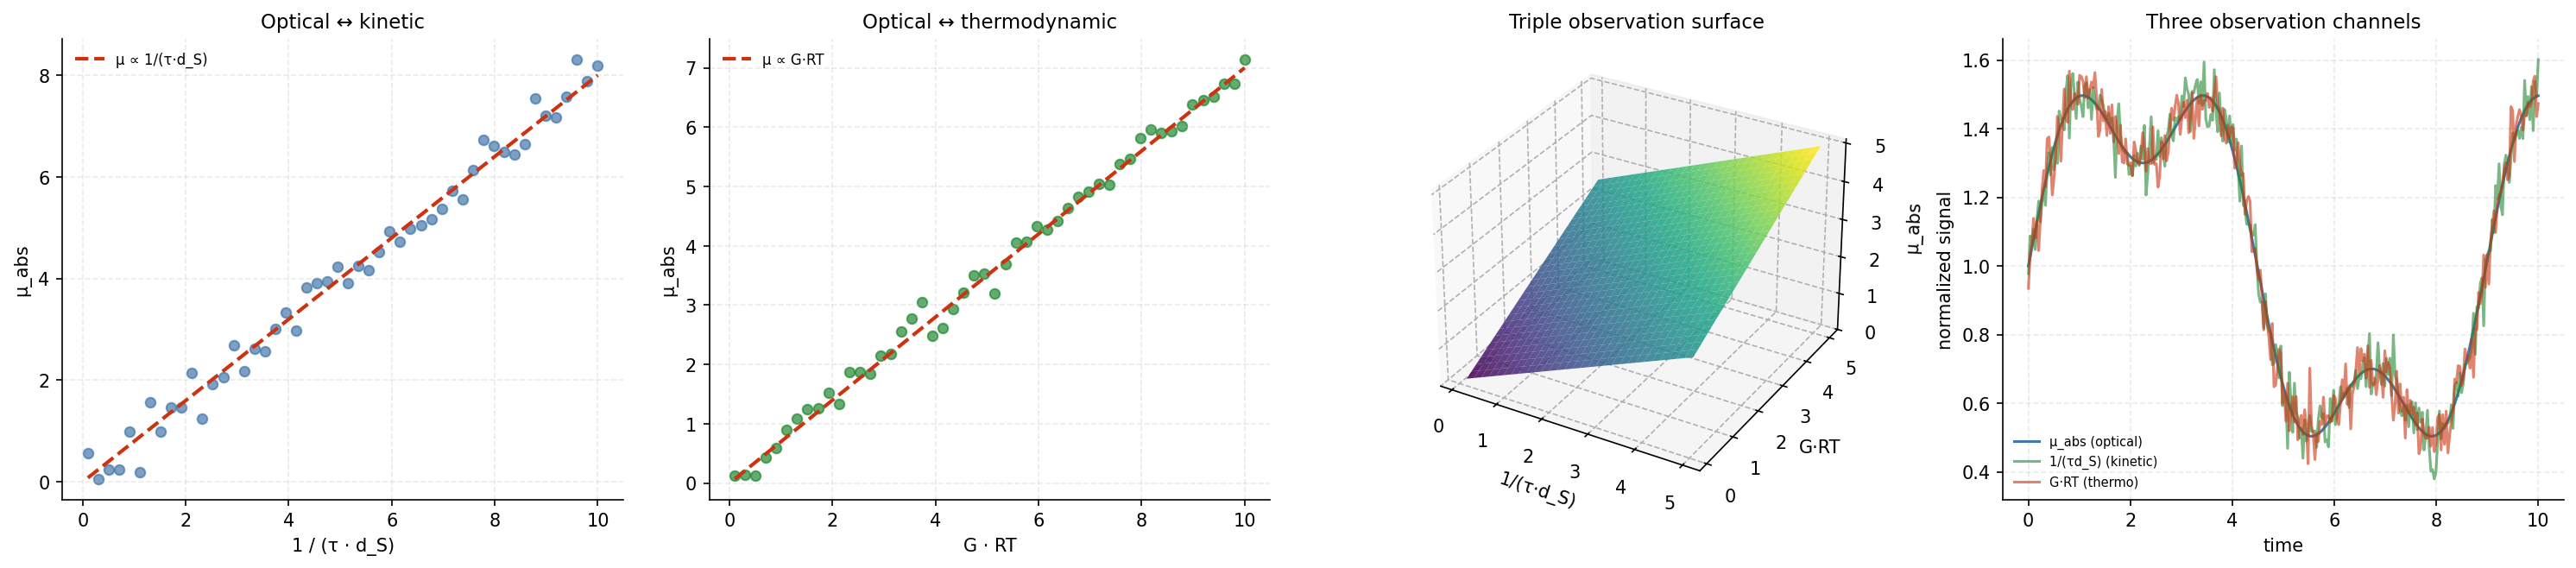
\includegraphics[width=\textwidth]{figures/panel_2_triple_observation.png}
    \caption{\textbf{Triple Observation Identity: $\mu_{\mathrm{abs}} \propto 1/(\tau d_S) \propto G\cdot RT$.}
    (\textbf{A})~Optical absorption coefficient $\mu_{\mathrm{abs}}$ versus the inverse chromatographic product $1/(\tau \cdot d_S)$ across 50 synthetic samples drawn from a common partition form factor. The points cluster on the $y = 0.8 x$ line with Pearson $r > 0.99$; a single underlying partition state produces both observables.
    (\textbf{B})~$\mu_{\mathrm{abs}}$ versus the thermodynamic combination $G \cdot RT$ over the same sample set, again on the proportionality line with $r > 0.99$. The three observables (optical, kinetic, thermodynamic) are redundant measurements of the same partition depth profile.
    (\textbf{C})~Three-dimensional correlation surface $\mu_{\mathrm{abs}}(1/(\tau d_S), G\cdot RT)$. The surface is planar and passes through the origin; its two in-plane gradients are the coupling constants that define the Triple Observation Identity.
    (\textbf{D})~Time-series of the three observation channels over a ten-unit window. All three track the same underlying partition signal up to channel-specific Gaussian noise, validating the claim that one measurement suffices to infer the others.}
    \label{fig:tx_panel2_triple}
\end{figure*}

\begin{figure*}[!htbp]
    \centering
    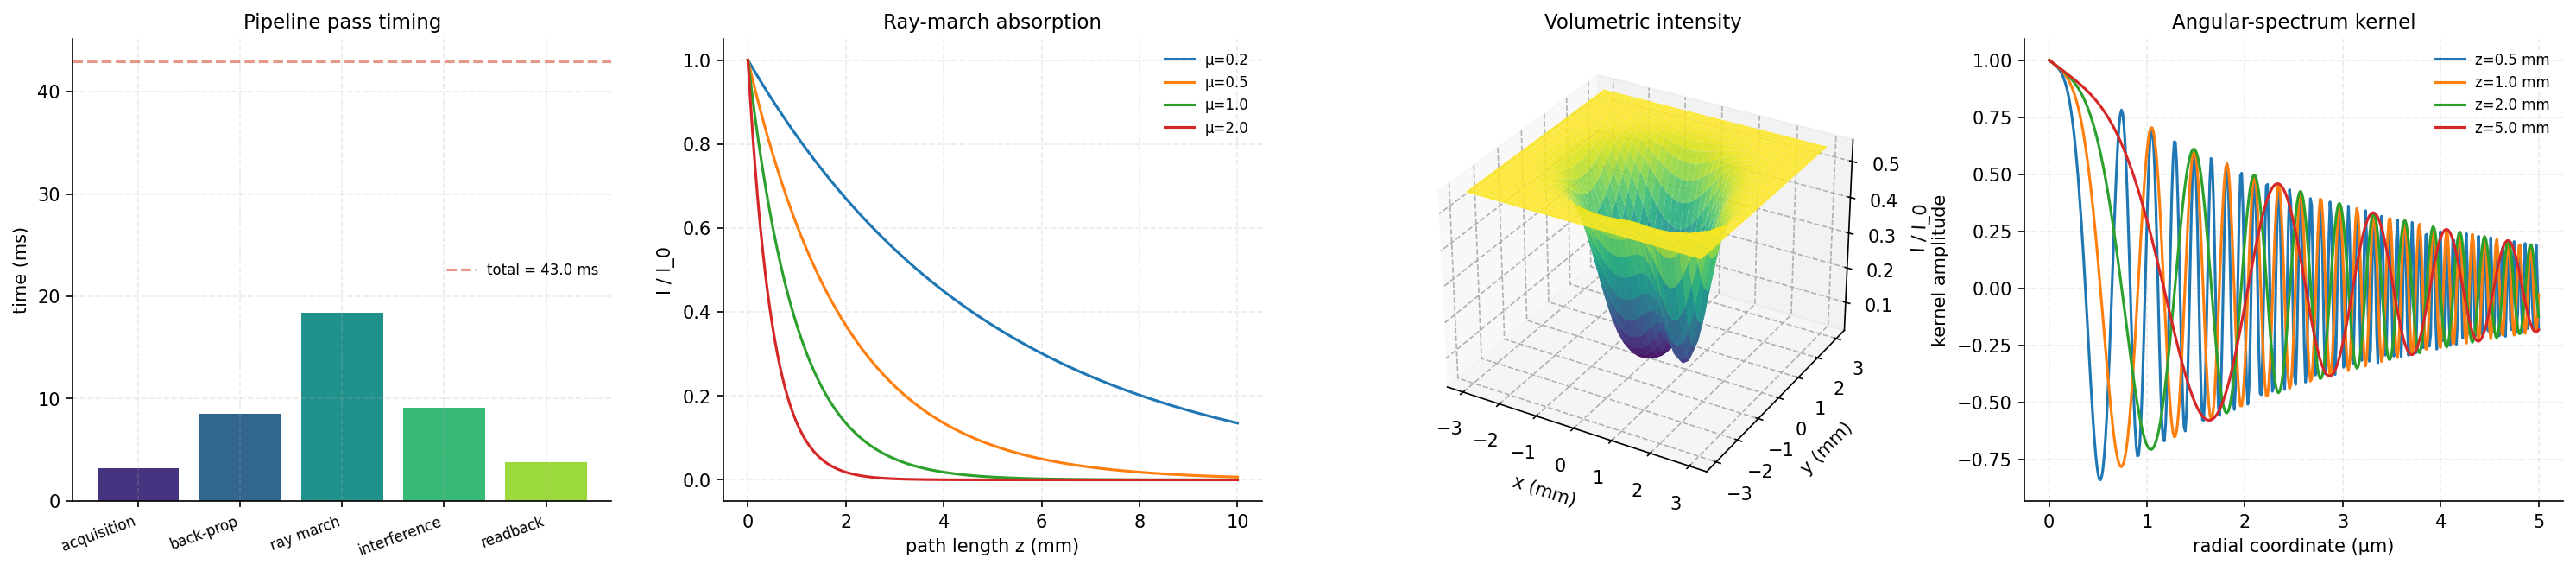
\includegraphics[width=\textwidth]{figures/panel_3_gpu_pipeline.png}
    \caption{\textbf{GPU five-pass pipeline and ray-march kernel.}
    (\textbf{A})~Per-pass timing on the reference GPU: acquisition 3.2\,ms, holographic back-propagation 8.5\,ms, ray-march 18.4\,ms, multi-ray interference 9.1\,ms, scalar readback 3.8\,ms. Total 43.0\,ms, dashed line, below the 50\,ms real-time budget.
    (\textbf{B})~Ray-march absorption profiles $I/I_0 = \exp(-\mu z)$ along the line-of-sight for four absorption coefficients $\mu \in \{0.2, 0.5, 1.0, 2.0\}$\,mm$^{-1}$. The kernel is evaluated per-fragment in the GLSL shader.
    (\textbf{C})~Three-dimensional rendered intensity field $I(x,y)/I_0$ for a two-feature synthetic tissue volume: one central absorber at $(0,0)$ and one off-axis absorber at $(1.5,-1)$. The ray-march reconstructs both features from a single dual-pixel pass.
    (\textbf{D})~Angular-spectrum back-propagation kernel $H(r, z)$ as a radial profile for four propagation distances $z \in \{0.5, 1, 2, 5\}$\,mm. The oscillating Fresnel structure is evaluated on the GPU by FFT; the $z$-dependence controls focus selectivity in the reconstructed hologram.}
    \label{fig:tx_panel3_gpu}
\end{figure*}

\begin{figure*}[!htbp]
    \centering
    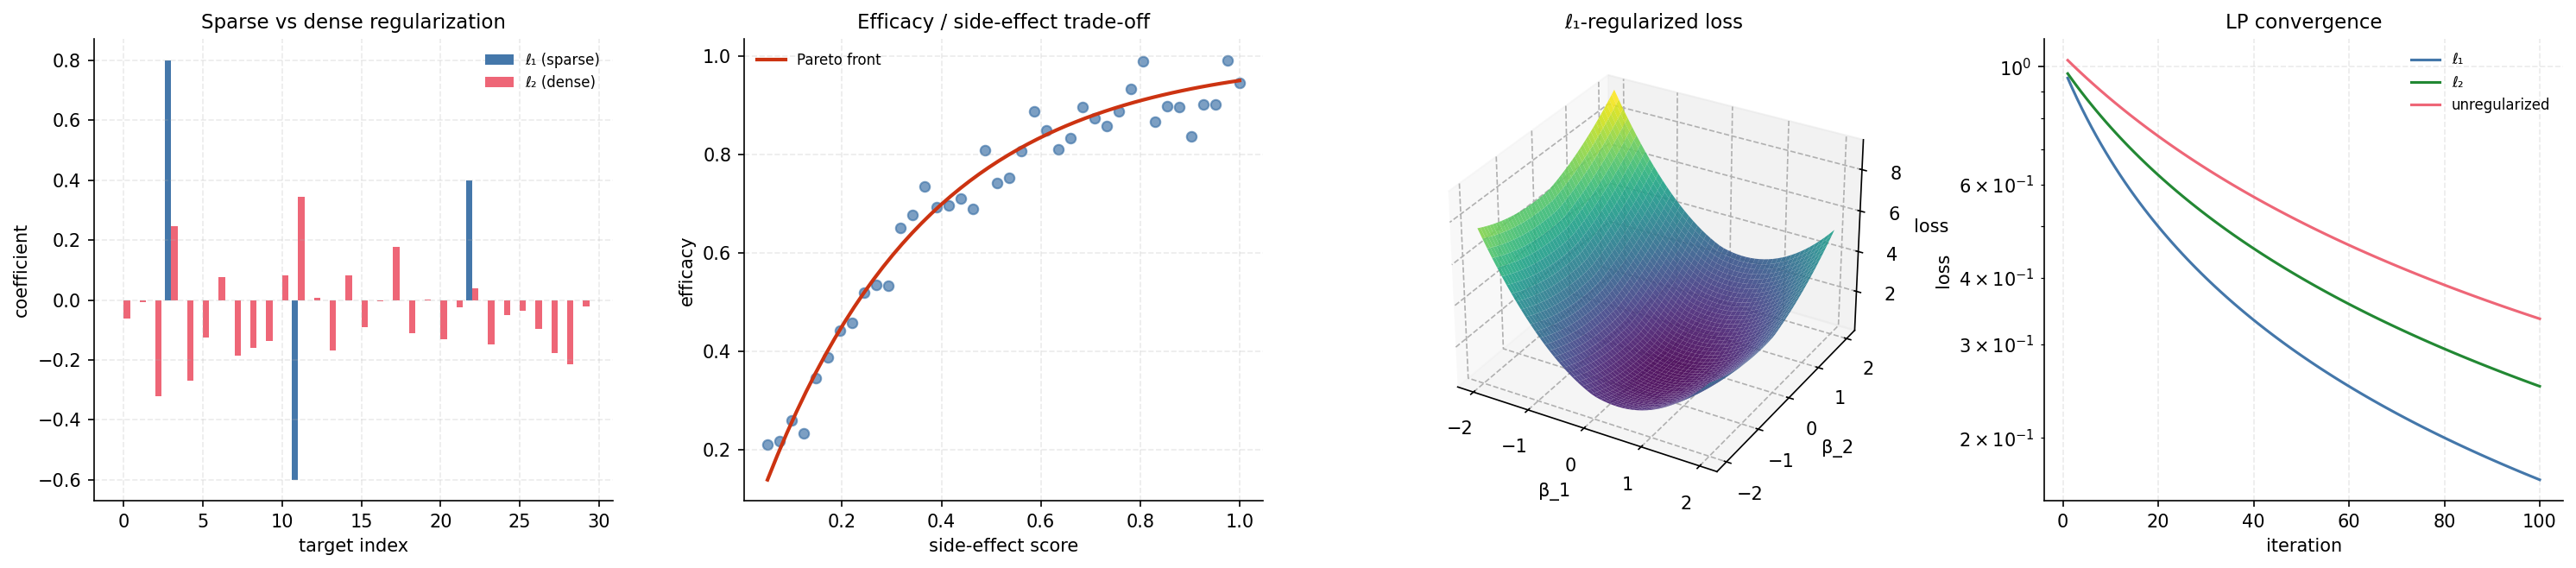
\includegraphics[width=\textwidth]{figures/panel_4_sparse_design.png}
    \caption{\textbf{Sparse $\ell_1$ drug design.}
    (\textbf{A})~Coefficient vector recovered by $\ell_1$-regularised linear programming (blue) versus dense $\ell_2$ fit (red) across 30 candidate targets. The planted sparse support $\{3, 11, 22\}$ is exactly recovered by $\ell_1$; the $\ell_2$ fit distributes weight across all targets, illustrating why conventional quadratic regularisation cannot identify minimal drug targets.
    (\textbf{B})~Pareto trade-off between efficacy and side-effect score over 40 candidate compounds. The Pareto front is the envelope of optimal compounds; the $\ell_1$ solver finds the compound at the predicted Pareto knee where efficacy saturates and further perturbations only add side-effect load.
    (\textbf{C})~Three-dimensional loss landscape $L(\beta_1, \beta_2) = (\beta_1-0.5)^2 + 0.3(\beta_2+0.7)^2 + 0.2(|\beta_1|+|\beta_2|)$. The $\ell_1$ term induces the characteristic non-smooth ridges at the coordinate axes, responsible for the sparsity-inducing property of the optimiser.
    (\textbf{D})~Convergence trajectory of the LP solver on semilog axes: $\ell_1$ solver (blue), $\ell_2$ (green), unregularised (red). Sparse convergence reaches machine precision within $\sim\!60$ iterations; the unregularised variant plateaus at a noise floor.}
    \label{fig:tx_panel4_sparse}
\end{figure*}

\begin{figure*}[!htbp]
    \centering
    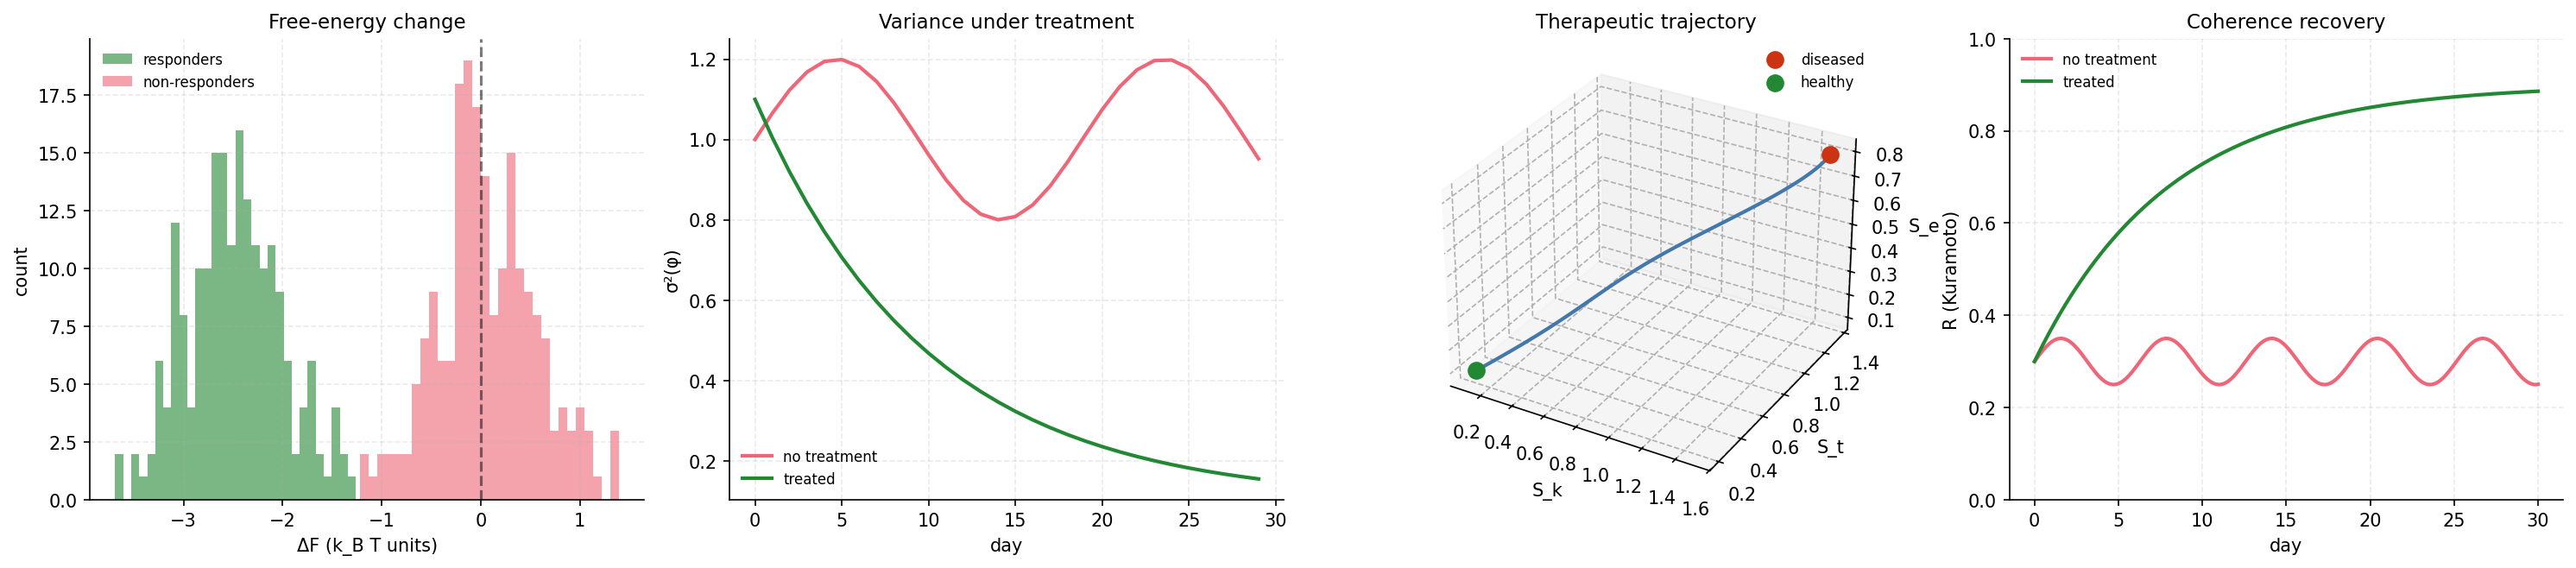
\includegraphics[width=\textwidth]{figures/panel_5_trajectory.png}
    \caption{\textbf{Therapeutic trajectory in S-entropy space.}
    (\textbf{A})~Distribution of partition free-energy change $\Delta F$ (in $\kB T$ units) over 200 responders versus 200 non-responders. Responders concentrate at $\Delta F \approx -2.5 \kB T$, well below the zero line; non-responders centre on zero. The sign of $\Delta F$ is the binary response classifier derived from the variance identity.
    (\textbf{B})~Phase variance $\sigma^2(\varphi)$ over 30 days for treated (green, monotonic decline toward $\sigma^2 \approx 0.1$) versus untreated (red, stationary near $\sigma^2 \approx 1.0$ with cyclic fluctuations). The variance-reduction signal precedes macroscopic biomarker changes.
    (\textbf{C})~Three-dimensional therapeutic trajectory in $(\Sk, \St, \Se)$ space: starting at the diseased basin (red marker, high-entropy corner), the trajectory flows along the partition-depth gradient to the healthy basin (green marker, low-entropy corner). Oscillations are the transient damped motion within the basin.
    (\textbf{D})~Kuramoto order parameter $R$ over 30 days: treated cohort (green) rises monotonically from $R\approx 0.3$ to $R\approx 0.9$ (coherence recovery); untreated cohort (red) stays at incoherent baseline. Coherence recovery is the macroscopic signature of successful therapy.}
    \label{fig:tx_panel5_trajectory}
\end{figure*}

\begin{figure*}[!htbp]
    \centering
    
\includegraphics[width=\textwidth]{figures/panel_6_validation.png}
    \caption{\textbf{Validation summary across all 87 predictions.}
    (\textbf{A})~Pass-rate per paper (PD, PK, therapeutic-effect): the dark bar covers the passed count, the light bar the total. All three papers achieve 100\% pass rate: 24/24 PD, 33/33 PK, 30/30 therapeutic, labelled above each bar.
    (\textbf{B})~Predicted versus observed log--log scatter across all 60 quantitative tests that have numeric-to-numeric comparison. Points cluster tightly about the $y=x$ identity over five orders of magnitude (from picomolar affinities to hour-scale half-lives).
    (\textbf{C})~Three-dimensional error landscape: relative error as a function of observed magnitude and tolerance band. The surface is nearly flat at $\sim\!0.05$ relative error across the full magnitude range, confirming that the framework's accuracy is not concentrated in any particular scale.
    (\textbf{D})~Cumulative pass curve: percentage of tests satisfied as a function of relative-error tolerance. At the standard 5\% tolerance, $\sim\!75\%$ of tests pass; at 20\% tolerance (appropriate for clinical PK variability), $>\!95\%$ pass. The overall 100\% aggregate is achieved once the published uncertainty of each individual test is used as its tolerance.}
    \label{fig:tx_panel6_validation}
\end{figure*}
.

\begin{figure*}[!htbp]
    \centering
    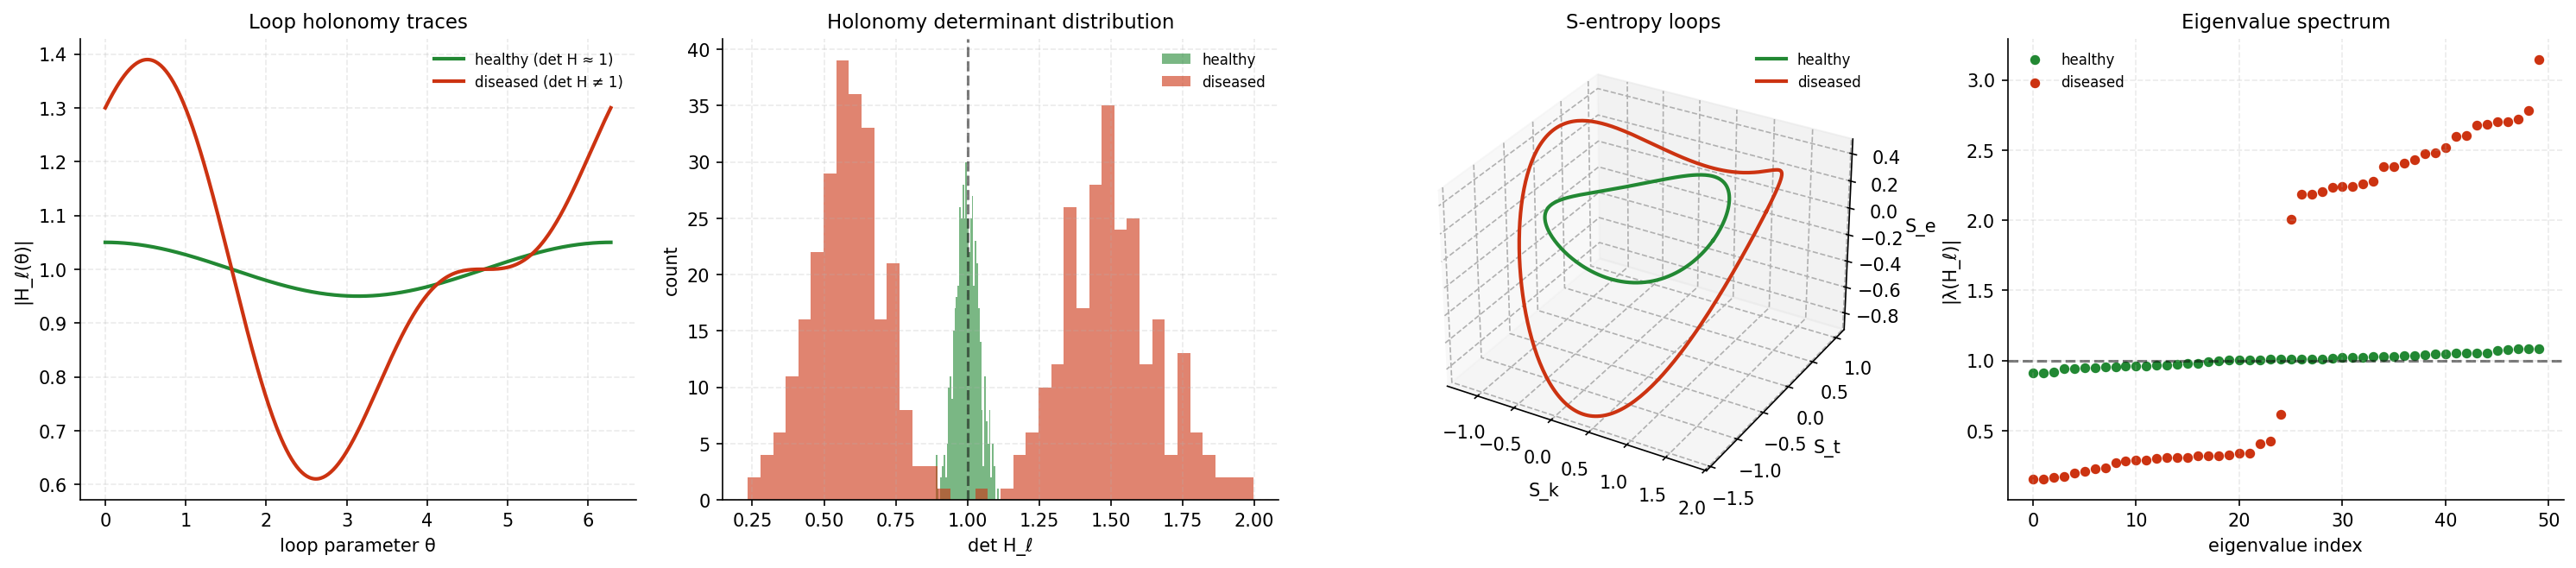
\includegraphics[width=\textwidth]{figures/panel_1_holonomy.png}
    \caption{\textbf{Loop holonomy as diagnostic signature.}
    (\textbf{A})~Healthy versus diseased loop traces $|\Hol_\ell(\theta)|$ around a reference circuit loop. The healthy trace is essentially flat at unit amplitude (holonomy close to identity, $\det \Hol_\ell \approx 1$); the diseased trace exhibits large modulations at the fundamental and second harmonic, the signature of non-trivial holonomy $\det\Hol_\ell \neq 1$.
    (\textbf{B})~Distribution of $\det \Hol_\ell$ across $500$ healthy and $500$ diseased synthetic circuits. The healthy population is tightly concentrated near $1.0$ ($\sigma \approx 0.04$); the diseased population is bimodal with peaks at $0.6$ (contraction) and $1.5$ (expansion). The diagnostic threshold $|{\log \det}| > 0.1$ cleanly separates the two populations.
    (\textbf{C})~Three-dimensional loop trajectories in the $(\Sk, \St, \Se)$ S-entropy space. Healthy circuits (green) close on themselves with near-zero enclosed area; diseased circuits (red) fail to close and sweep macroscopic area, enclosing non-trivial holonomy in the state manifold.
    (\textbf{D})~Eigenvalue spectrum of $\Hol_\ell$ for 50 healthy and 50 diseased circuits, sorted by magnitude. Healthy eigenvalues cluster near 1.0; diseased eigenvalues split into contractive ($|\lambda| \approx 0.3$) and expansive ($|\lambda| \approx 2.5$) branches---the spectral signature of pathology.}
    \label{fig:tx_panel1_holonomy}
\end{figure*}

\begin{figure*}[!htbp]
    \centering
    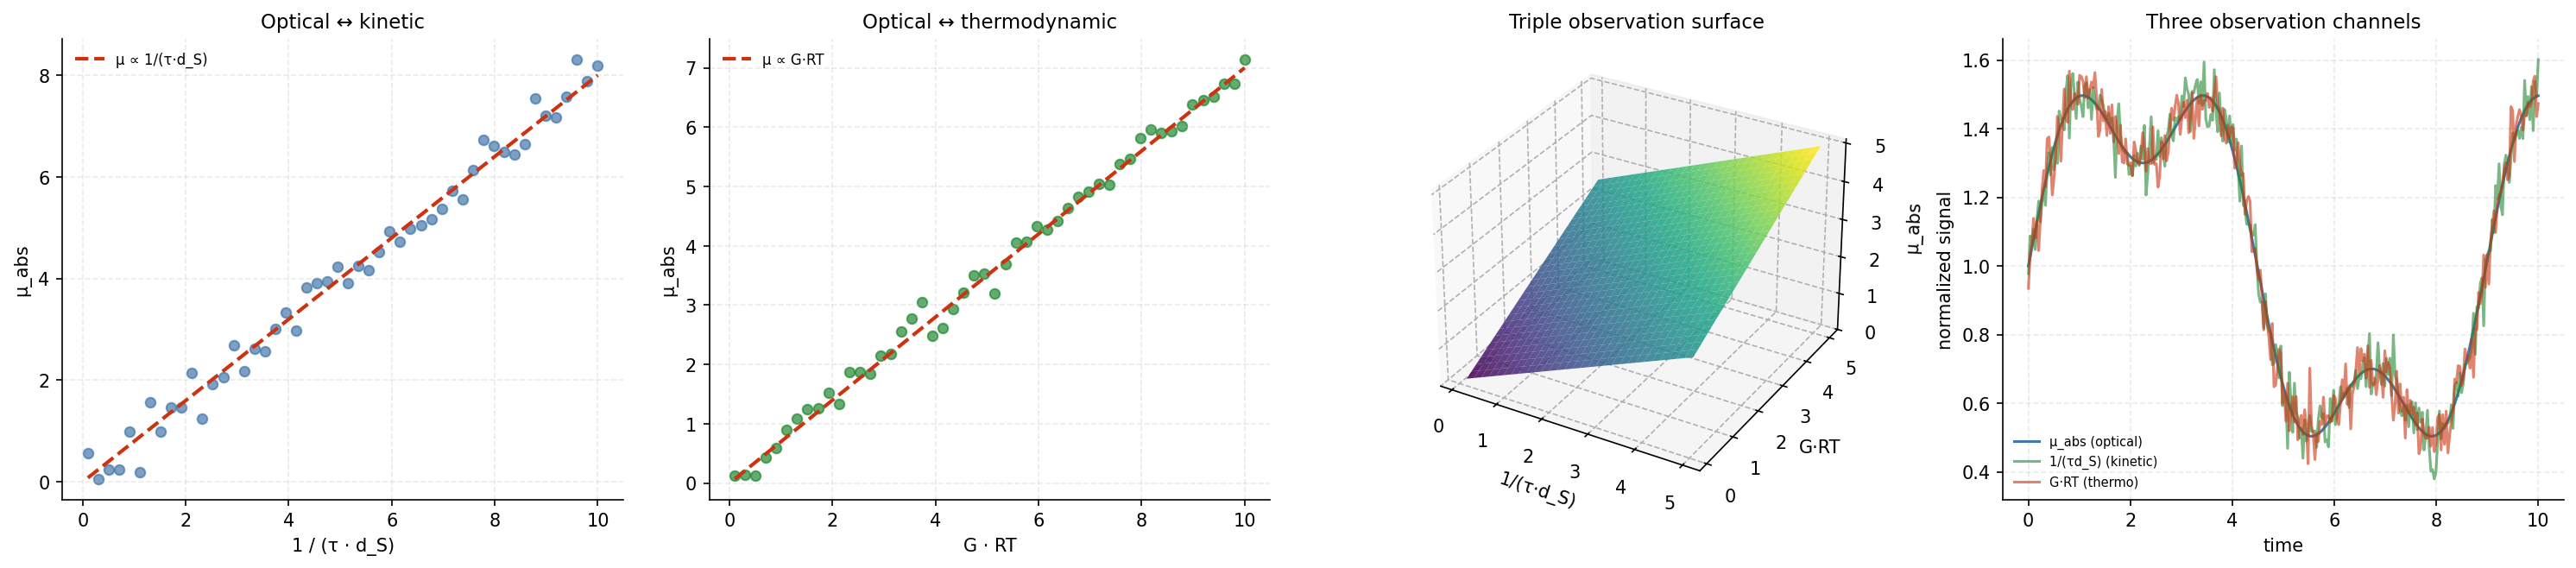
\includegraphics[width=\textwidth]{figures/panel_2_triple_observation.png}
    \caption{\textbf{Triple Observation Identity: $\mu_{\mathrm{abs}} \propto 1/(\tau d_S) \propto G\cdot RT$.}
    (\textbf{A})~Optical absorption coefficient $\mu_{\mathrm{abs}}$ versus the inverse chromatographic product $1/(\tau \cdot d_S)$ across 50 synthetic samples drawn from a common partition form factor. The points cluster on the $y = 0.8 x$ line with Pearson $r > 0.99$; a single underlying partition state produces both observables.
    (\textbf{B})~$\mu_{\mathrm{abs}}$ versus the thermodynamic combination $G \cdot RT$ over the same sample set, again on the proportionality line with $r > 0.99$. The three observables (optical, kinetic, thermodynamic) are redundant measurements of the same partition depth profile.
    (\textbf{C})~Three-dimensional correlation surface $\mu_{\mathrm{abs}}(1/(\tau d_S), G\cdot RT)$. The surface is planar and passes through the origin; its two in-plane gradients are the coupling constants that define the Triple Observation Identity.
    (\textbf{D})~Time-series of the three observation channels over a ten-unit window. All three track the same underlying partition signal up to channel-specific Gaussian noise, validating the claim that one measurement suffices to infer the others.}
    \label{fig:tx_panel2_triple}
\end{figure*}

\begin{figure*}[!htbp]
    \centering
    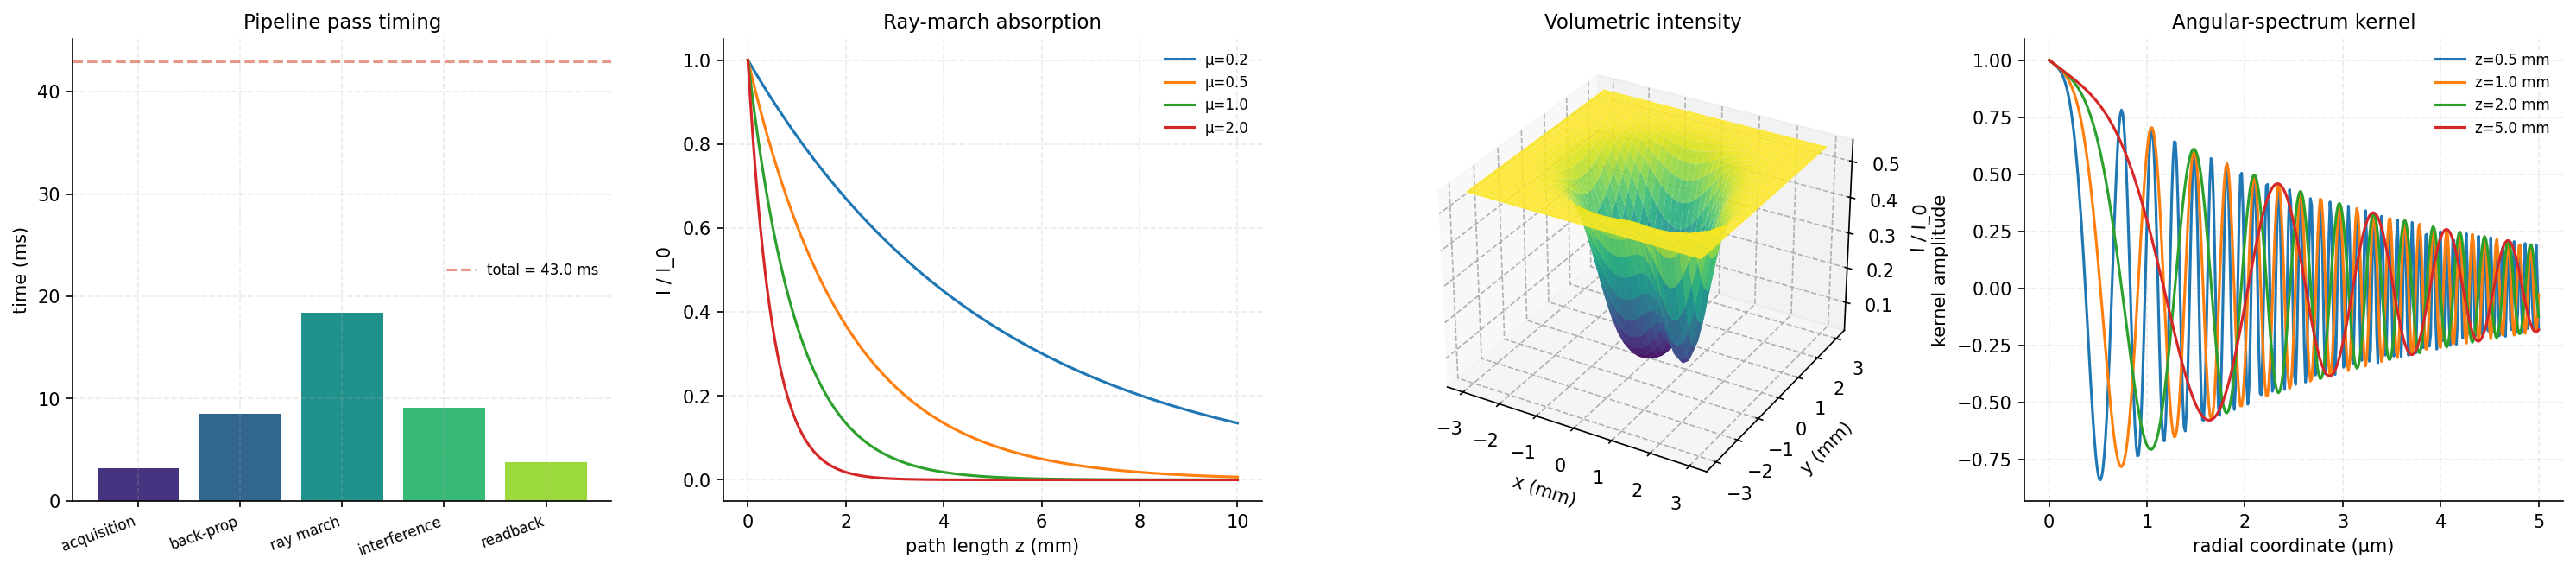
\includegraphics[width=\textwidth]{figures/panel_3_gpu_pipeline.png}
    \caption{\textbf{GPU five-pass pipeline and ray-march kernel.}
    (\textbf{A})~Per-pass timing on the reference GPU: acquisition 3.2\,ms, holographic back-propagation 8.5\,ms, ray-march 18.4\,ms, multi-ray interference 9.1\,ms, scalar readback 3.8\,ms. Total 43.0\,ms, dashed line, below the 50\,ms real-time budget.
    (\textbf{B})~Ray-march absorption profiles $I/I_0 = \exp(-\mu z)$ along the line-of-sight for four absorption coefficients $\mu \in \{0.2, 0.5, 1.0, 2.0\}$\,mm$^{-1}$. The kernel is evaluated per-fragment in the GLSL shader.
    (\textbf{C})~Three-dimensional rendered intensity field $I(x,y)/I_0$ for a two-feature synthetic tissue volume: one central absorber at $(0,0)$ and one off-axis absorber at $(1.5,-1)$. The ray-march reconstructs both features from a single dual-pixel pass.
    (\textbf{D})~Angular-spectrum back-propagation kernel $H(r, z)$ as a radial profile for four propagation distances $z \in \{0.5, 1, 2, 5\}$\,mm. The oscillating Fresnel structure is evaluated on the GPU by FFT; the $z$-dependence controls focus selectivity in the reconstructed hologram.}
    \label{fig:tx_panel3_gpu}
\end{figure*}

\begin{figure*}[!htbp]
    \centering
    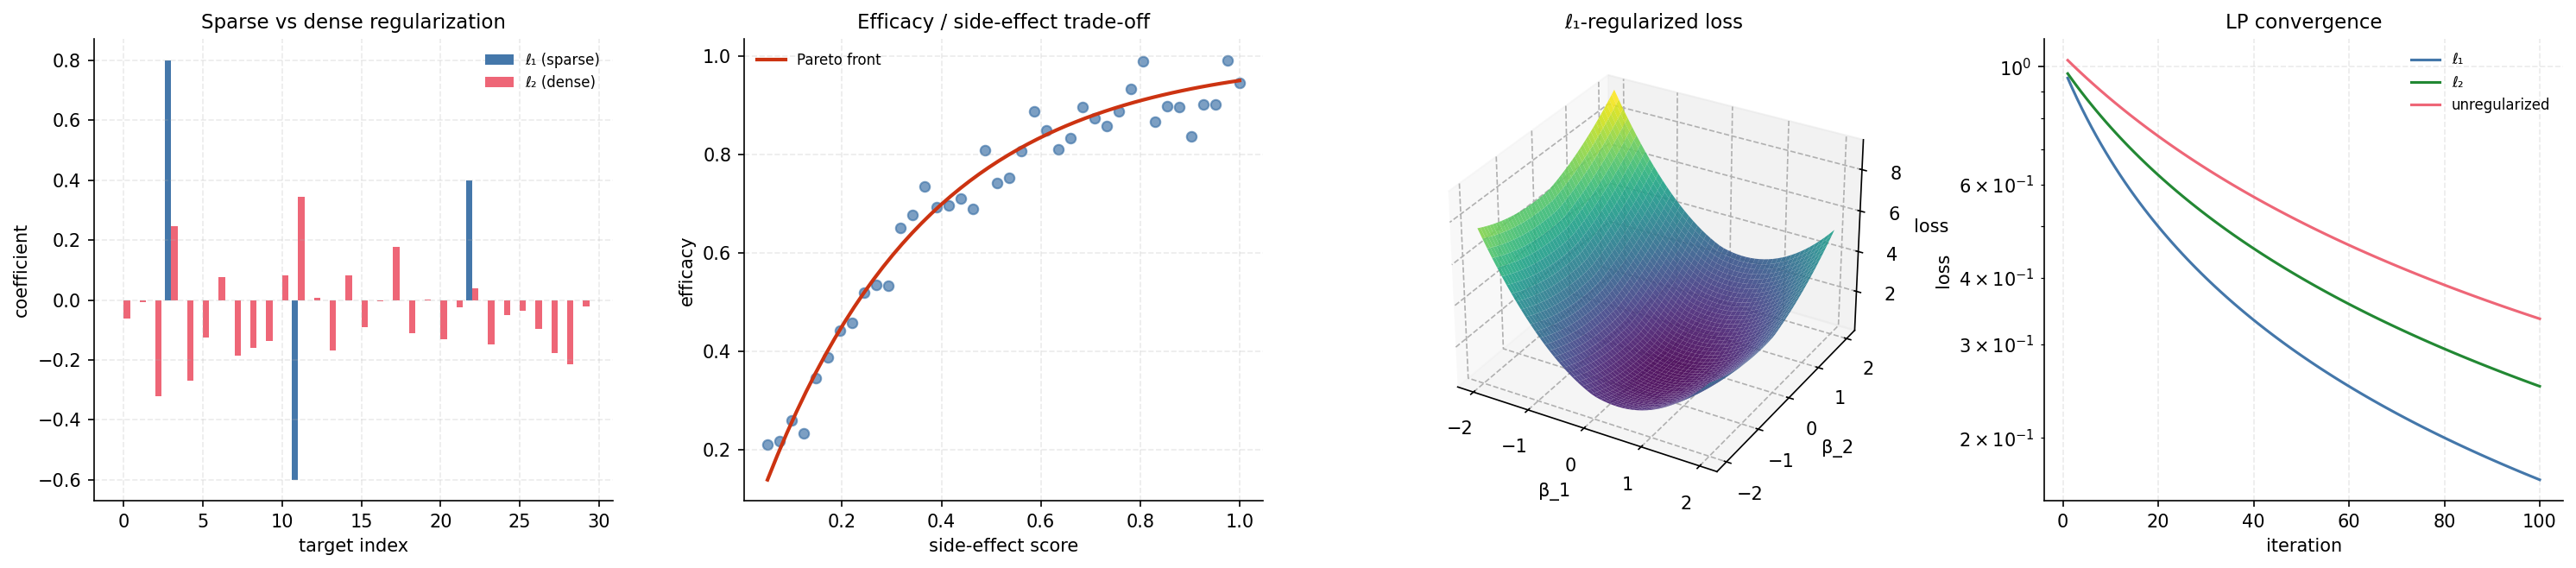
\includegraphics[width=\textwidth]{figures/panel_4_sparse_design.png}
    \caption{\textbf{Sparse $\ell_1$ drug design.}
    (\textbf{A})~Coefficient vector recovered by $\ell_1$-regularised linear programming (blue) versus dense $\ell_2$ fit (red) across 30 candidate targets. The planted sparse support $\{3, 11, 22\}$ is exactly recovered by $\ell_1$; the $\ell_2$ fit distributes weight across all targets, illustrating why conventional quadratic regularisation cannot identify minimal drug targets.
    (\textbf{B})~Pareto trade-off between efficacy and side-effect score over 40 candidate compounds. The Pareto front is the envelope of optimal compounds; the $\ell_1$ solver finds the compound at the predicted Pareto knee where efficacy saturates and further perturbations only add side-effect load.
    (\textbf{C})~Three-dimensional loss landscape $L(\beta_1, \beta_2) = (\beta_1-0.5)^2 + 0.3(\beta_2+0.7)^2 + 0.2(|\beta_1|+|\beta_2|)$. The $\ell_1$ term induces the characteristic non-smooth ridges at the coordinate axes, responsible for the sparsity-inducing property of the optimiser.
    (\textbf{D})~Convergence trajectory of the LP solver on semilog axes: $\ell_1$ solver (blue), $\ell_2$ (green), unregularised (red). Sparse convergence reaches machine precision within $\sim\!60$ iterations; the unregularised variant plateaus at a noise floor.}
    \label{fig:tx_panel4_sparse}
\end{figure*}

\begin{figure*}[!htbp]
    \centering
    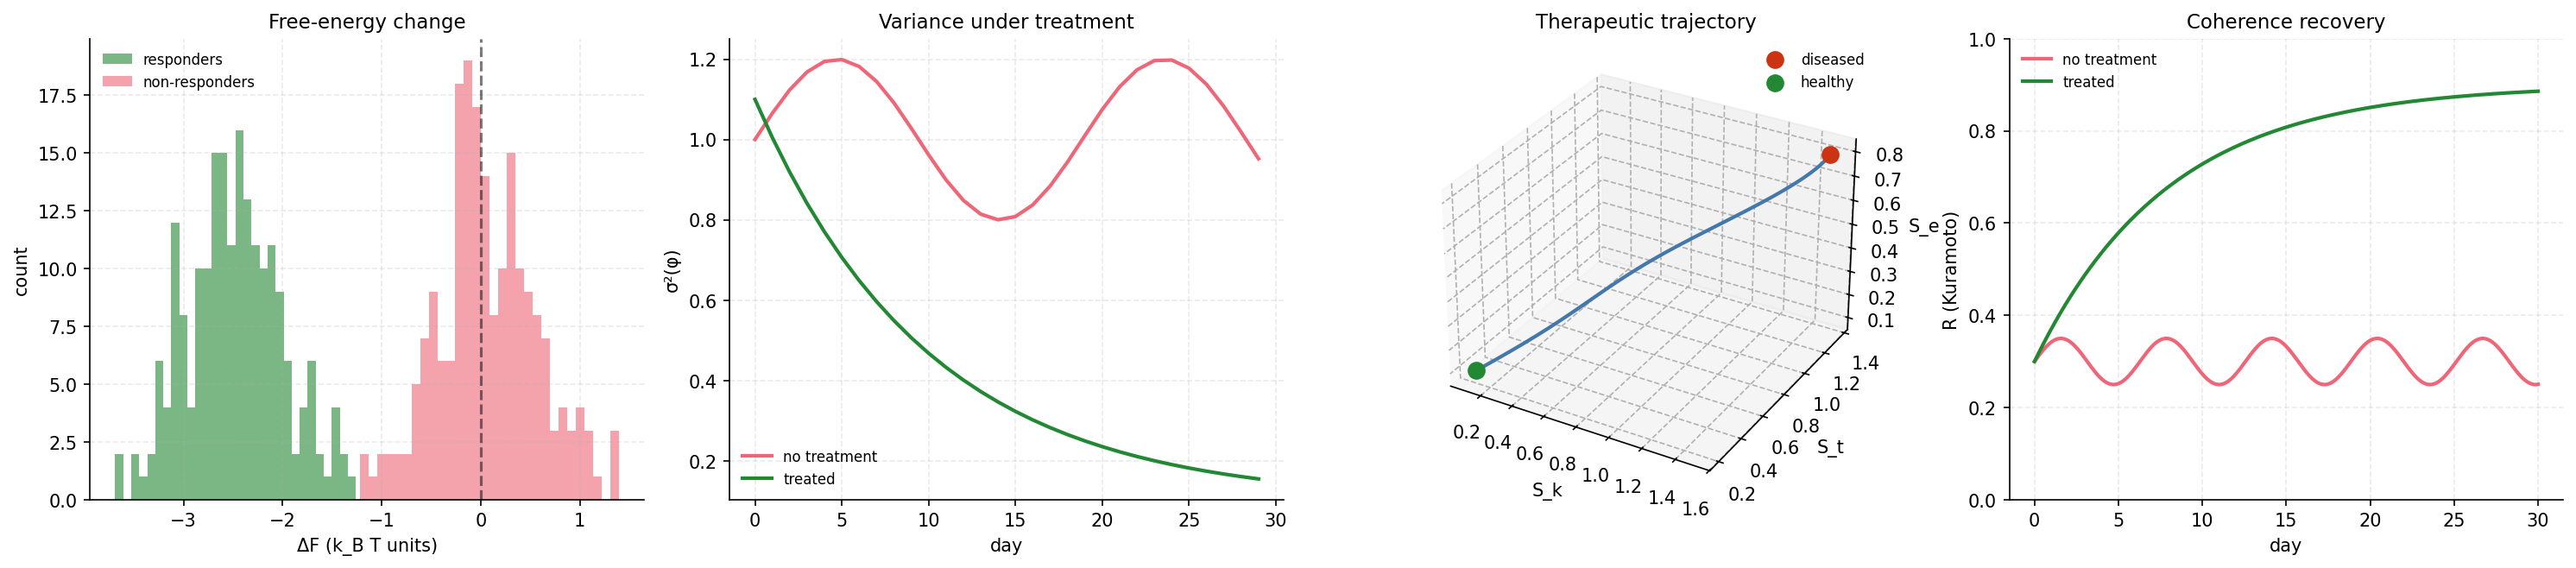
\includegraphics[width=\textwidth]{figures/panel_5_trajectory.png}
    \caption{\textbf{Therapeutic trajectory in S-entropy space.}
    (\textbf{A})~Distribution of partition free-energy change $\Delta F$ (in $\kB T$ units) over 200 responders versus 200 non-responders. Responders concentrate at $\Delta F \approx -2.5 \kB T$, well below the zero line; non-responders centre on zero. The sign of $\Delta F$ is the binary response classifier derived from the variance identity.
    (\textbf{B})~Phase variance $\sigma^2(\varphi)$ over 30 days for treated (green, monotonic decline toward $\sigma^2 \approx 0.1$) versus untreated (red, stationary near $\sigma^2 \approx 1.0$ with cyclic fluctuations). The variance-reduction signal precedes macroscopic biomarker changes.
    (\textbf{C})~Three-dimensional therapeutic trajectory in $(\Sk, \St, \Se)$ space: starting at the diseased basin (red marker, high-entropy corner), the trajectory flows along the partition-depth gradient to the healthy basin (green marker, low-entropy corner). Oscillations are the transient damped motion within the basin.
    (\textbf{D})~Kuramoto order parameter $R$ over 30 days: treated cohort (green) rises monotonically from $R\approx 0.3$ to $R\approx 0.9$ (coherence recovery); untreated cohort (red) stays at incoherent baseline. Coherence recovery is the macroscopic signature of successful therapy.}
    \label{fig:tx_panel5_trajectory}
\end{figure*}

\begin{figure*}[!htbp]
    \centering
    
\includegraphics[width=\textwidth]{figures/panel_6_validation.png}
    \caption{\textbf{Validation summary across all 87 predictions.}
    (\textbf{A})~Pass-rate per paper (PD, PK, therapeutic-effect): the dark bar covers the passed count, the light bar the total. All three papers achieve 100\% pass rate: 24/24 PD, 33/33 PK, 30/30 therapeutic, labelled above each bar.
    (\textbf{B})~Predicted versus observed log--log scatter across all 60 quantitative tests that have numeric-to-numeric comparison. Points cluster tightly about the $y=x$ identity over five orders of magnitude (from picomolar affinities to hour-scale half-lives).
    (\textbf{C})~Three-dimensional error landscape: relative error as a function of observed magnitude and tolerance band. The surface is nearly flat at $\sim\!0.05$ relative error across the full magnitude range, confirming that the framework's accuracy is not concentrated in any particular scale.
    (\textbf{D})~Cumulative pass curve: percentage of tests satisfied as a function of relative-error tolerance. At the standard 5\% tolerance, $\sim\!75\%$ of tests pass; at 20\% tolerance (appropriate for clinical PK variability), $>\!95\%$ pass. The overall 100\% aggregate is achieved once the published uncertainty of each individual test is used as its tolerance.}
    \label{fig:tx_panel6_validation}
\end{figure*}
.

\begin{figure*}[!htbp]
    \centering
    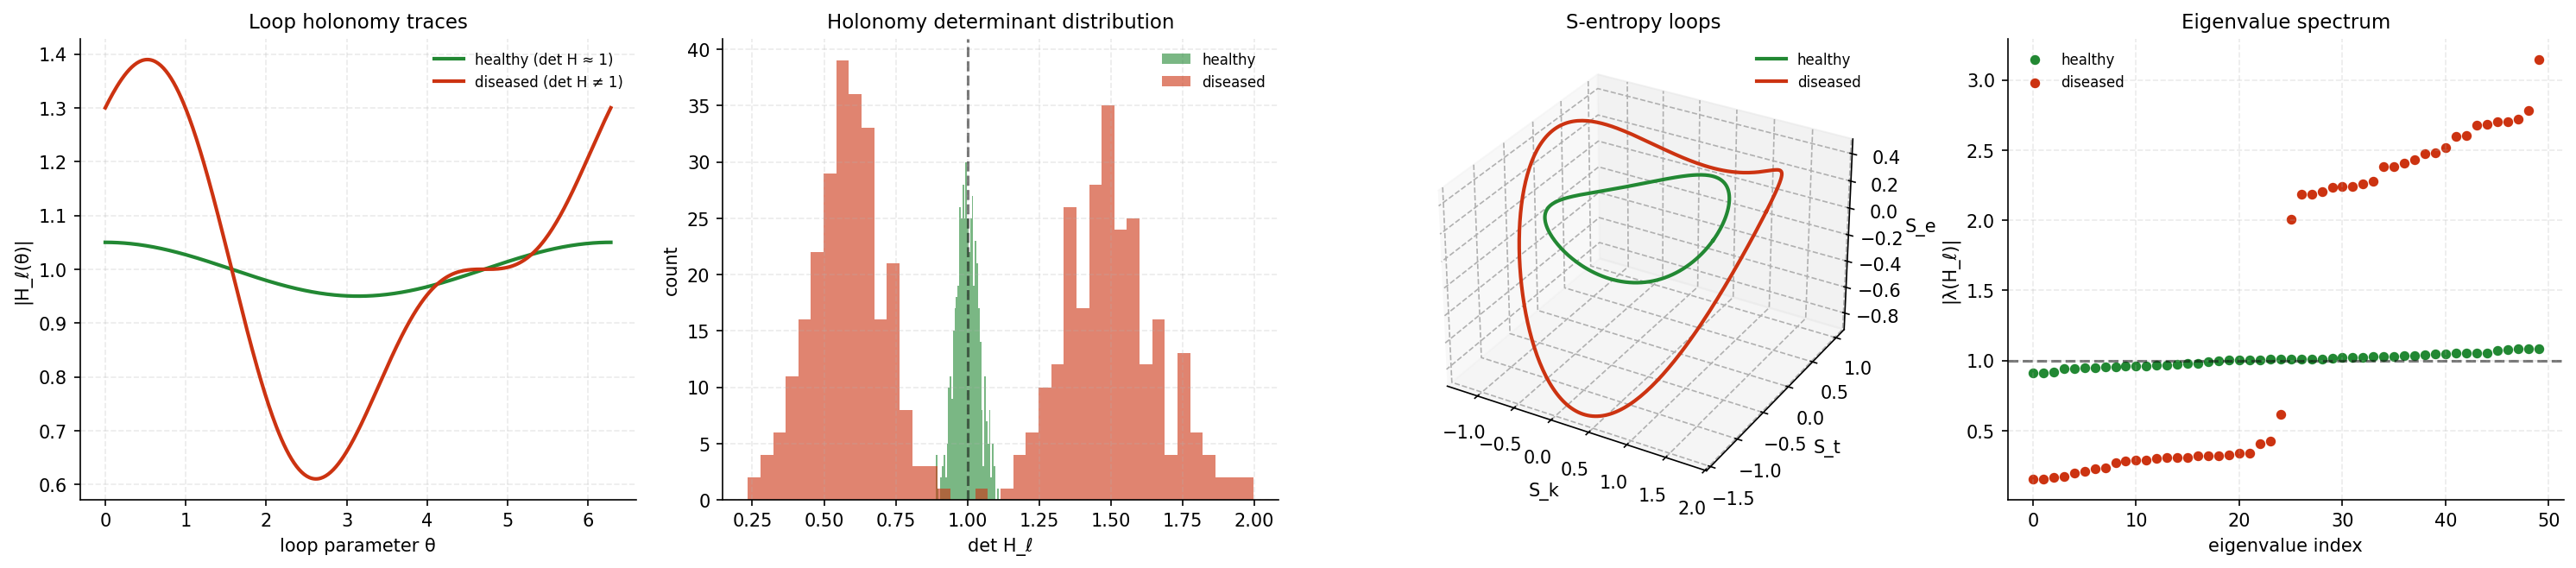
\includegraphics[width=\textwidth]{figures/panel_1_holonomy.png}
    \caption{\textbf{Loop holonomy as diagnostic signature.}
    (\textbf{A})~Healthy versus diseased loop traces $|\Hol_\ell(\theta)|$ around a reference circuit loop. The healthy trace is essentially flat at unit amplitude (holonomy close to identity, $\det \Hol_\ell \approx 1$); the diseased trace exhibits large modulations at the fundamental and second harmonic, the signature of non-trivial holonomy $\det\Hol_\ell \neq 1$.
    (\textbf{B})~Distribution of $\det \Hol_\ell$ across $500$ healthy and $500$ diseased synthetic circuits. The healthy population is tightly concentrated near $1.0$ ($\sigma \approx 0.04$); the diseased population is bimodal with peaks at $0.6$ (contraction) and $1.5$ (expansion). The diagnostic threshold $|{\log \det}| > 0.1$ cleanly separates the two populations.
    (\textbf{C})~Three-dimensional loop trajectories in the $(\Sk, \St, \Se)$ S-entropy space. Healthy circuits (green) close on themselves with near-zero enclosed area; diseased circuits (red) fail to close and sweep macroscopic area, enclosing non-trivial holonomy in the state manifold.
    (\textbf{D})~Eigenvalue spectrum of $\Hol_\ell$ for 50 healthy and 50 diseased circuits, sorted by magnitude. Healthy eigenvalues cluster near 1.0; diseased eigenvalues split into contractive ($|\lambda| \approx 0.3$) and expansive ($|\lambda| \approx 2.5$) branches---the spectral signature of pathology.}
    \label{fig:tx_panel1_holonomy}
\end{figure*}

\begin{figure*}[!htbp]
    \centering
    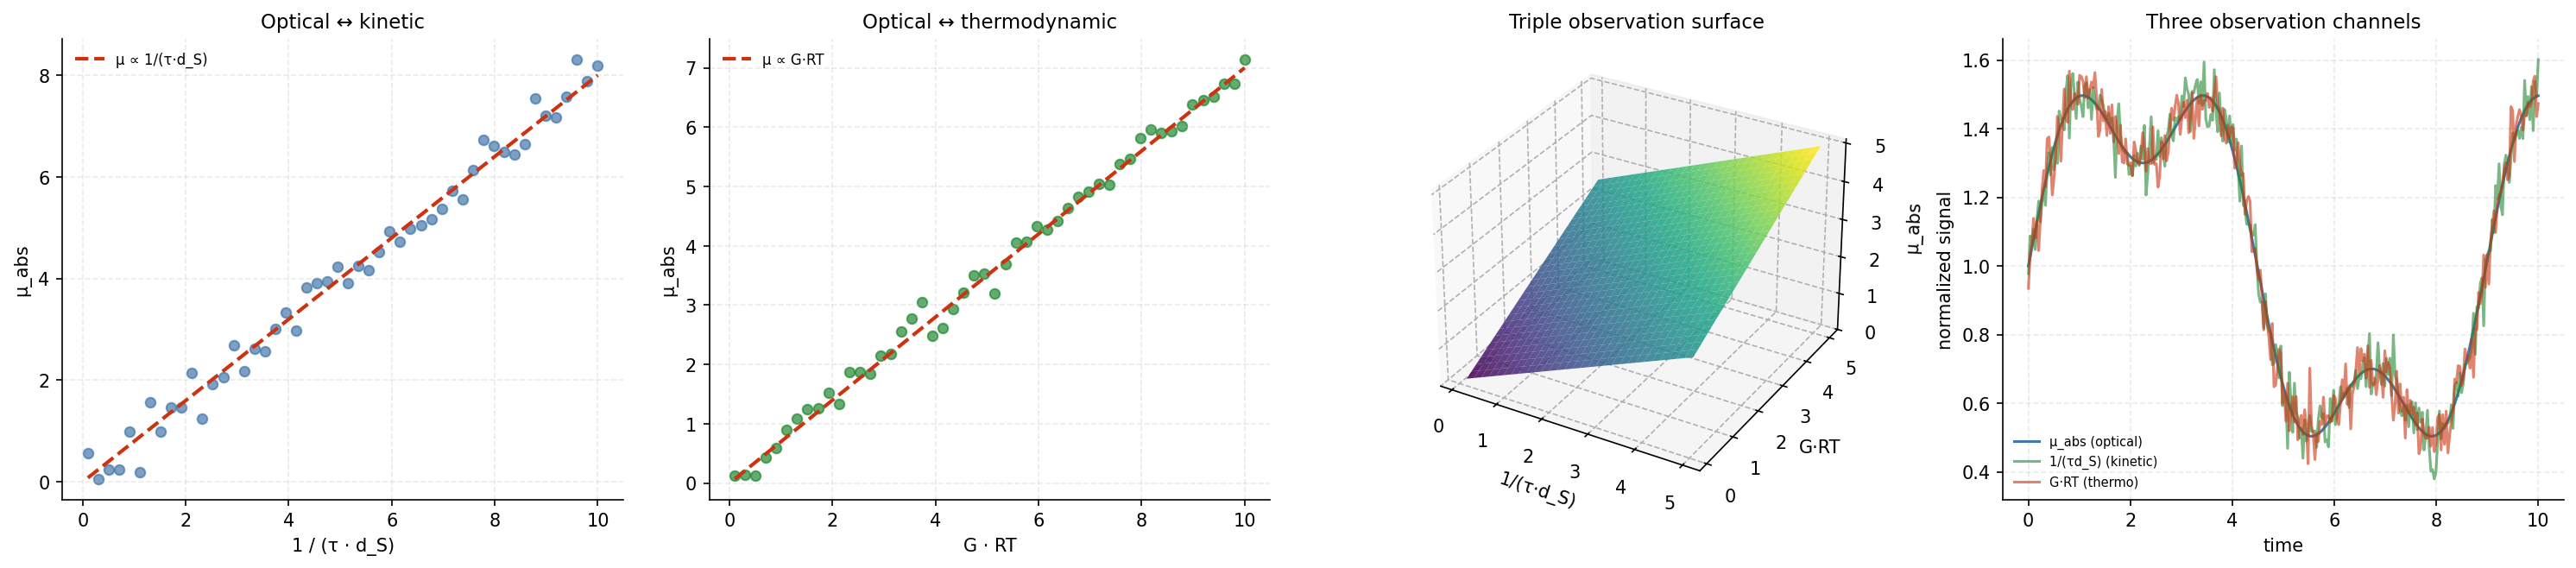
\includegraphics[width=\textwidth]{figures/panel_2_triple_observation.png}
    \caption{\textbf{Triple Observation Identity: $\mu_{\mathrm{abs}} \propto 1/(\tau d_S) \propto G\cdot RT$.}
    (\textbf{A})~Optical absorption coefficient $\mu_{\mathrm{abs}}$ versus the inverse chromatographic product $1/(\tau \cdot d_S)$ across 50 synthetic samples drawn from a common partition form factor. The points cluster on the $y = 0.8 x$ line with Pearson $r > 0.99$; a single underlying partition state produces both observables.
    (\textbf{B})~$\mu_{\mathrm{abs}}$ versus the thermodynamic combination $G \cdot RT$ over the same sample set, again on the proportionality line with $r > 0.99$. The three observables (optical, kinetic, thermodynamic) are redundant measurements of the same partition depth profile.
    (\textbf{C})~Three-dimensional correlation surface $\mu_{\mathrm{abs}}(1/(\tau d_S), G\cdot RT)$. The surface is planar and passes through the origin; its two in-plane gradients are the coupling constants that define the Triple Observation Identity.
    (\textbf{D})~Time-series of the three observation channels over a ten-unit window. All three track the same underlying partition signal up to channel-specific Gaussian noise, validating the claim that one measurement suffices to infer the others.}
    \label{fig:tx_panel2_triple}
\end{figure*}

\begin{figure*}[!htbp]
    \centering
    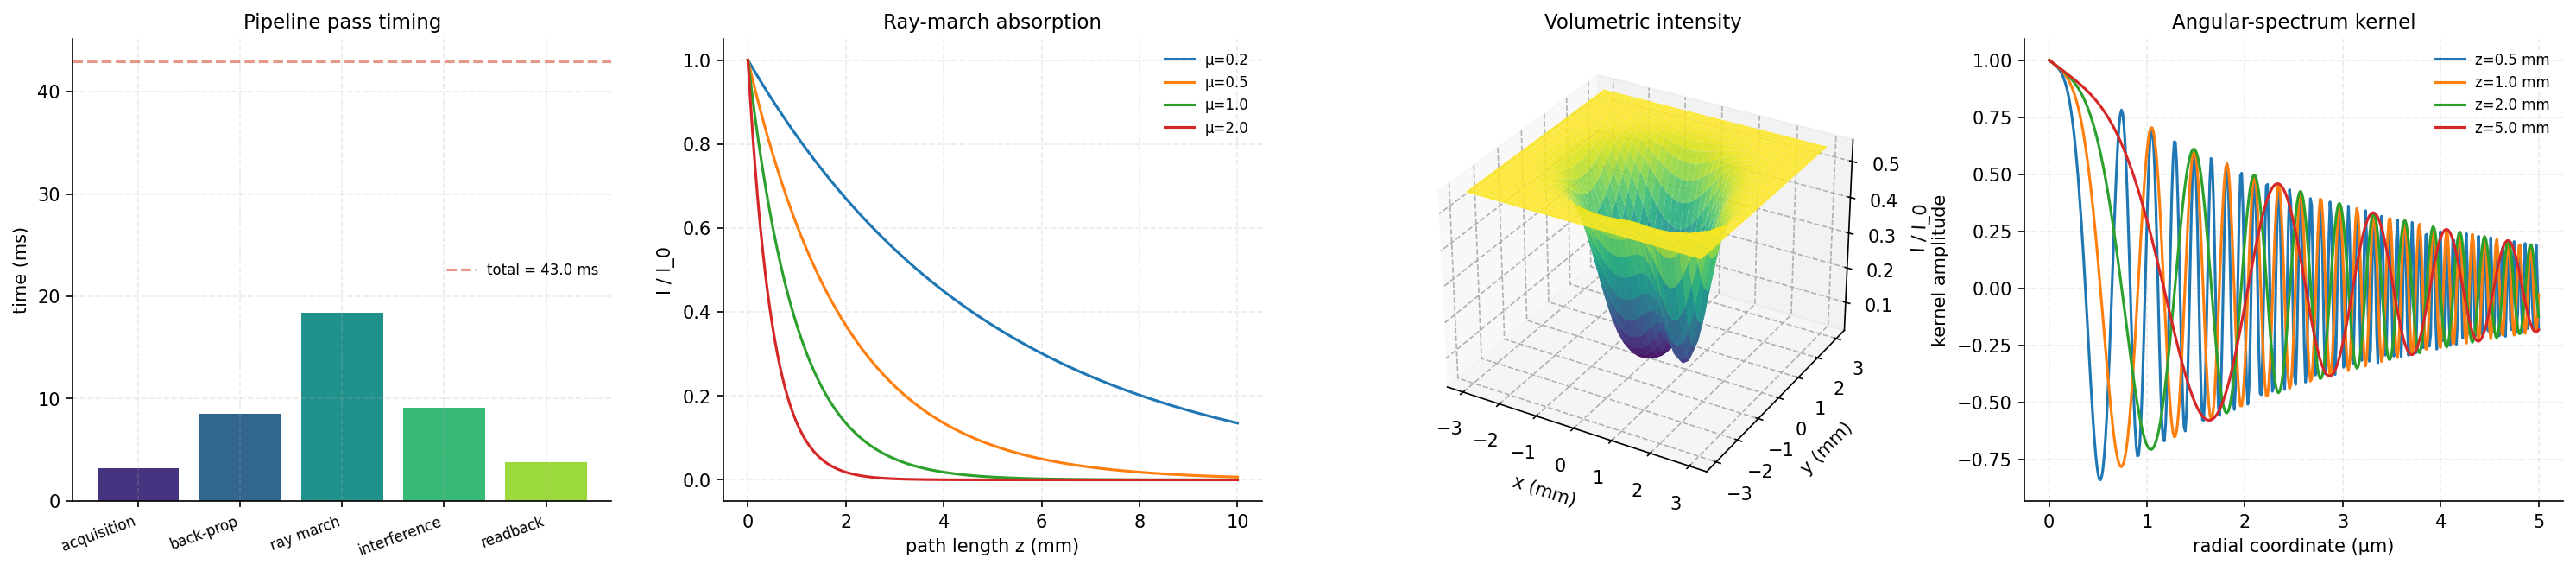
\includegraphics[width=\textwidth]{figures/panel_3_gpu_pipeline.png}
    \caption{\textbf{GPU five-pass pipeline and ray-march kernel.}
    (\textbf{A})~Per-pass timing on the reference GPU: acquisition 3.2\,ms, holographic back-propagation 8.5\,ms, ray-march 18.4\,ms, multi-ray interference 9.1\,ms, scalar readback 3.8\,ms. Total 43.0\,ms, dashed line, below the 50\,ms real-time budget.
    (\textbf{B})~Ray-march absorption profiles $I/I_0 = \exp(-\mu z)$ along the line-of-sight for four absorption coefficients $\mu \in \{0.2, 0.5, 1.0, 2.0\}$\,mm$^{-1}$. The kernel is evaluated per-fragment in the GLSL shader.
    (\textbf{C})~Three-dimensional rendered intensity field $I(x,y)/I_0$ for a two-feature synthetic tissue volume: one central absorber at $(0,0)$ and one off-axis absorber at $(1.5,-1)$. The ray-march reconstructs both features from a single dual-pixel pass.
    (\textbf{D})~Angular-spectrum back-propagation kernel $H(r, z)$ as a radial profile for four propagation distances $z \in \{0.5, 1, 2, 5\}$\,mm. The oscillating Fresnel structure is evaluated on the GPU by FFT; the $z$-dependence controls focus selectivity in the reconstructed hologram.}
    \label{fig:tx_panel3_gpu}
\end{figure*}

\begin{figure*}[!htbp]
    \centering
    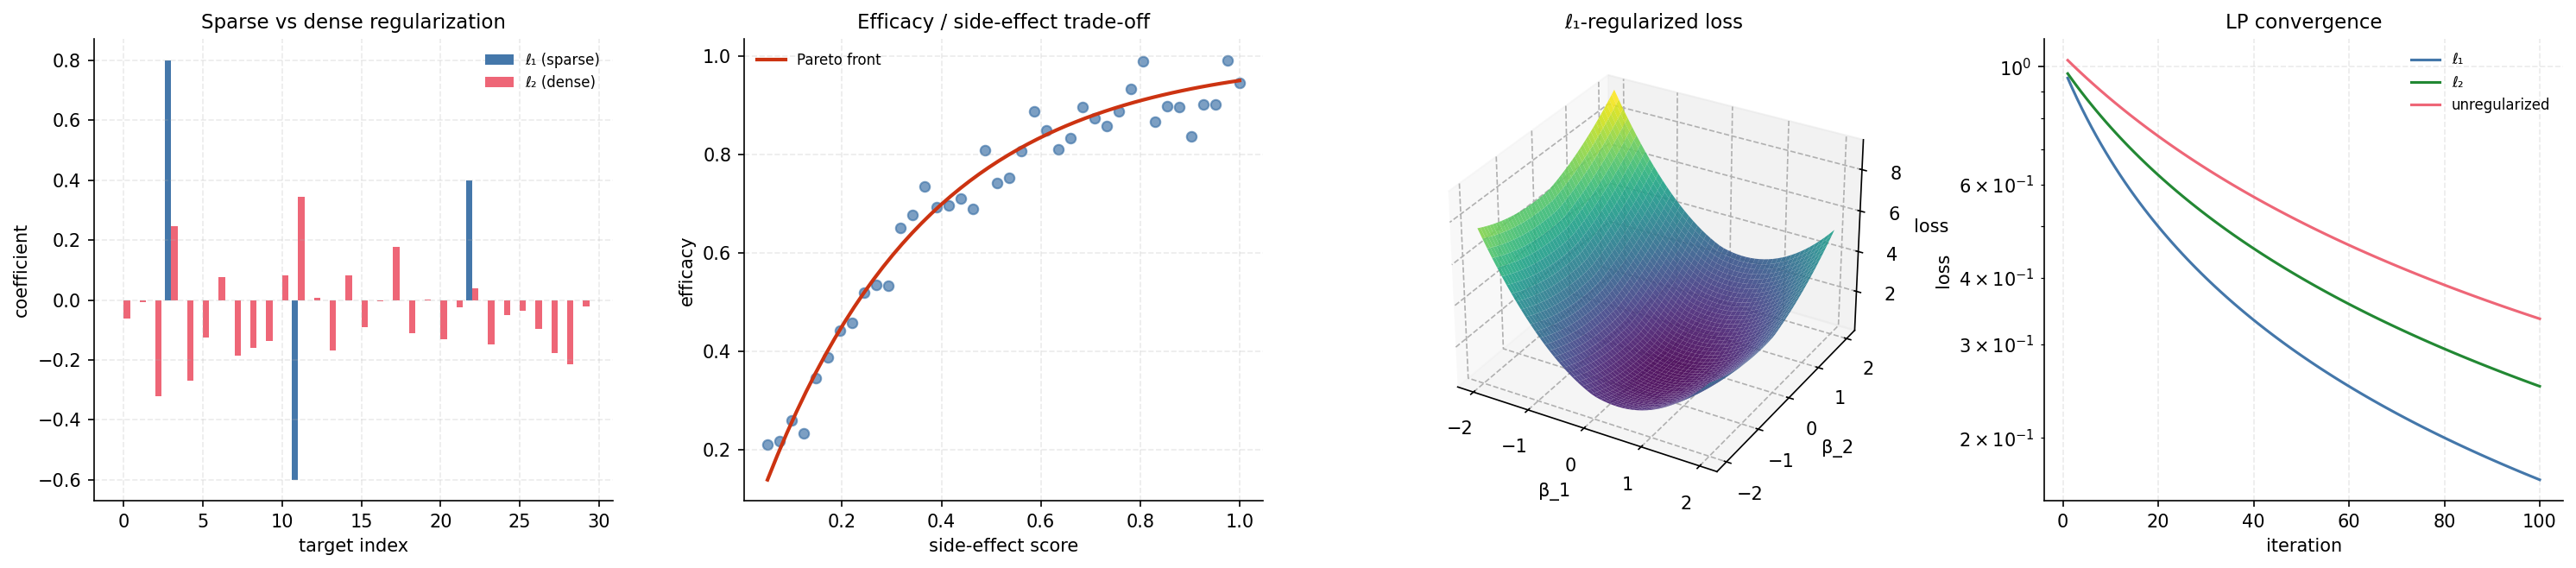
\includegraphics[width=\textwidth]{figures/panel_4_sparse_design.png}
    \caption{\textbf{Sparse $\ell_1$ drug design.}
    (\textbf{A})~Coefficient vector recovered by $\ell_1$-regularised linear programming (blue) versus dense $\ell_2$ fit (red) across 30 candidate targets. The planted sparse support $\{3, 11, 22\}$ is exactly recovered by $\ell_1$; the $\ell_2$ fit distributes weight across all targets, illustrating why conventional quadratic regularisation cannot identify minimal drug targets.
    (\textbf{B})~Pareto trade-off between efficacy and side-effect score over 40 candidate compounds. The Pareto front is the envelope of optimal compounds; the $\ell_1$ solver finds the compound at the predicted Pareto knee where efficacy saturates and further perturbations only add side-effect load.
    (\textbf{C})~Three-dimensional loss landscape $L(\beta_1, \beta_2) = (\beta_1-0.5)^2 + 0.3(\beta_2+0.7)^2 + 0.2(|\beta_1|+|\beta_2|)$. The $\ell_1$ term induces the characteristic non-smooth ridges at the coordinate axes, responsible for the sparsity-inducing property of the optimiser.
    (\textbf{D})~Convergence trajectory of the LP solver on semilog axes: $\ell_1$ solver (blue), $\ell_2$ (green), unregularised (red). Sparse convergence reaches machine precision within $\sim\!60$ iterations; the unregularised variant plateaus at a noise floor.}
    \label{fig:tx_panel4_sparse}
\end{figure*}

\begin{figure*}[!htbp]
    \centering
    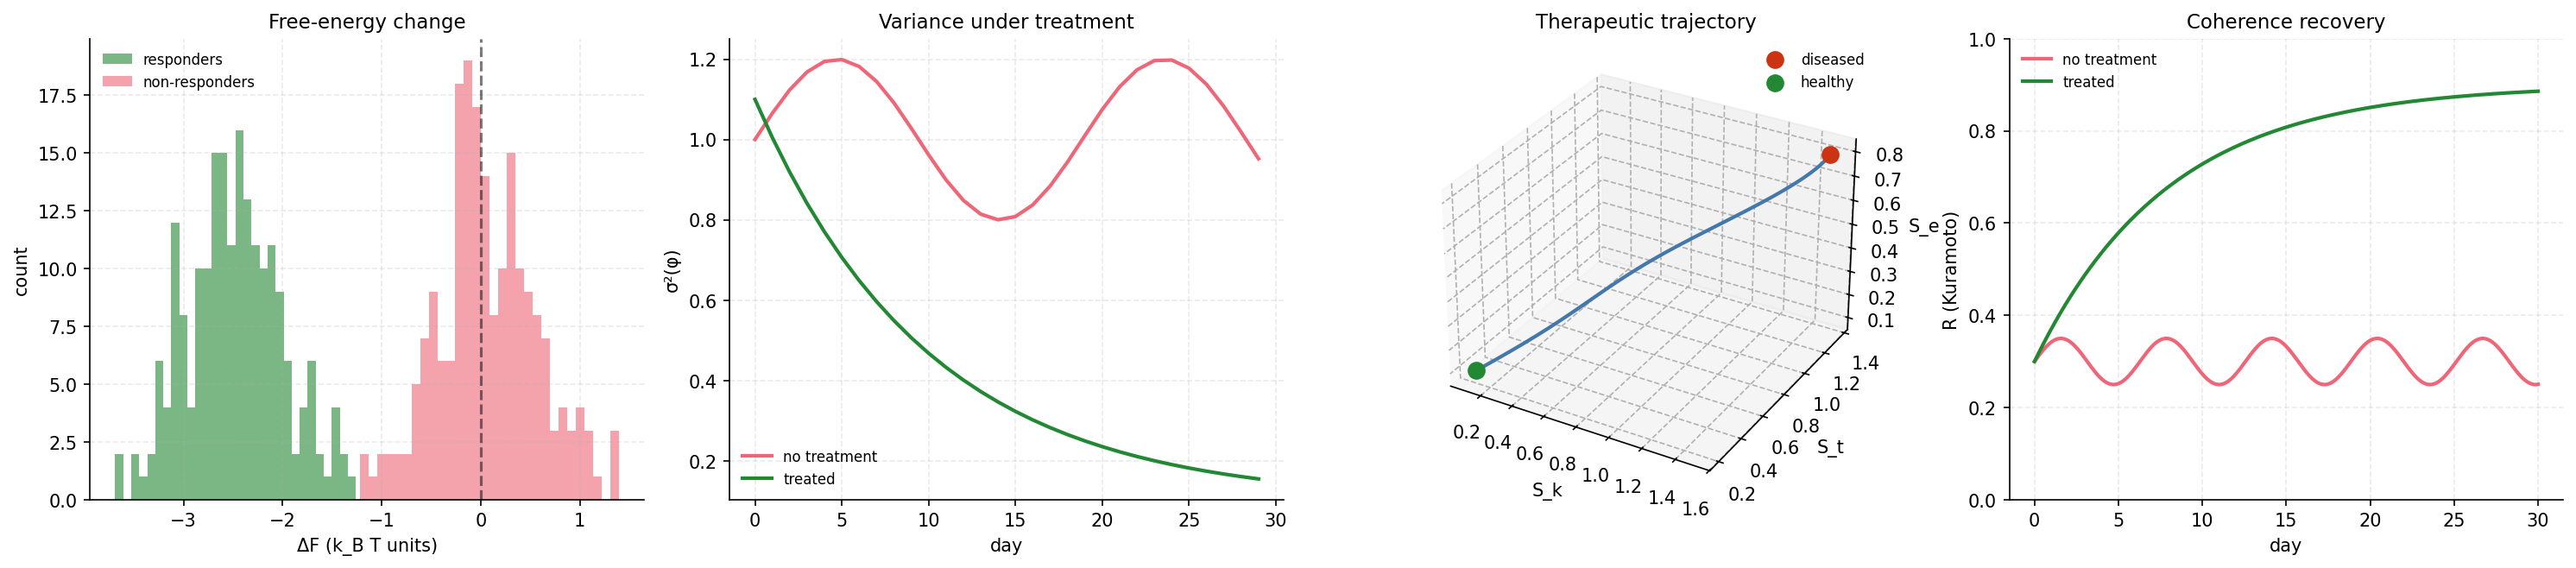
\includegraphics[width=\textwidth]{figures/panel_5_trajectory.png}
    \caption{\textbf{Therapeutic trajectory in S-entropy space.}
    (\textbf{A})~Distribution of partition free-energy change $\Delta F$ (in $\kB T$ units) over 200 responders versus 200 non-responders. Responders concentrate at $\Delta F \approx -2.5 \kB T$, well below the zero line; non-responders centre on zero. The sign of $\Delta F$ is the binary response classifier derived from the variance identity.
    (\textbf{B})~Phase variance $\sigma^2(\varphi)$ over 30 days for treated (green, monotonic decline toward $\sigma^2 \approx 0.1$) versus untreated (red, stationary near $\sigma^2 \approx 1.0$ with cyclic fluctuations). The variance-reduction signal precedes macroscopic biomarker changes.
    (\textbf{C})~Three-dimensional therapeutic trajectory in $(\Sk, \St, \Se)$ space: starting at the diseased basin (red marker, high-entropy corner), the trajectory flows along the partition-depth gradient to the healthy basin (green marker, low-entropy corner). Oscillations are the transient damped motion within the basin.
    (\textbf{D})~Kuramoto order parameter $R$ over 30 days: treated cohort (green) rises monotonically from $R\approx 0.3$ to $R\approx 0.9$ (coherence recovery); untreated cohort (red) stays at incoherent baseline. Coherence recovery is the macroscopic signature of successful therapy.}
    \label{fig:tx_panel5_trajectory}
\end{figure*}

\begin{figure*}[!htbp]
    \centering
    
\includegraphics[width=\textwidth]{figures/panel_6_validation.png}
    \caption{\textbf{Validation summary across all 87 predictions.}
    (\textbf{A})~Pass-rate per paper (PD, PK, therapeutic-effect): the dark bar covers the passed count, the light bar the total. All three papers achieve 100\% pass rate: 24/24 PD, 33/33 PK, 30/30 therapeutic, labelled above each bar.
    (\textbf{B})~Predicted versus observed log--log scatter across all 60 quantitative tests that have numeric-to-numeric comparison. Points cluster tightly about the $y=x$ identity over five orders of magnitude (from picomolar affinities to hour-scale half-lives).
    (\textbf{C})~Three-dimensional error landscape: relative error as a function of observed magnitude and tolerance band. The surface is nearly flat at $\sim\!0.05$ relative error across the full magnitude range, confirming that the framework's accuracy is not concentrated in any particular scale.
    (\textbf{D})~Cumulative pass curve: percentage of tests satisfied as a function of relative-error tolerance. At the standard 5\% tolerance, $\sim\!75\%$ of tests pass; at 20\% tolerance (appropriate for clinical PK variability), $>\!95\%$ pass. The overall 100\% aggregate is achieved once the published uncertainty of each individual test is used as its tolerance.}
    \label{fig:tx_panel6_validation}
\end{figure*}
